%    minted language=cpp,

%%%%%%
%%%%%%%%%%%%%%%%%%%%%%%%%%%%%% Title Page Info %%%%%%%%%%%%%%%%%%%%%%%%%%%%%%%%%%%%%%%%%%%
%%%%%%%%%%%%%%%%%%%%%%%%%%%%%%%%%%%%%%%%%%%%%%%%%%%%%%%%%%%%%%%%%%%%%%%%%%%%%%%%%%%%%%%%%%

\documentclass[aspectratio=169,compress]{beamer}
\mode<presentation> 

\usetheme{Warsaw}
\usecolortheme[rgb={0.7,0.0,0.0}]{structure}


\usepackage[algosection,lined]{algorithm2e}
\usepackage{minted}
\usepackage{tcolorbox}
\tcbuselibrary{minted}


% define
%\usepackage{beamerouterthememiniframes} % Para los puntitos 
\setbeamertemplate{footline}[frame number]{}

% include packages
\usepackage{subfigure}
\usepackage{multicol}
\usepackage{amsmath}
\usepackage{epsfig}
\usepackage{graphicx}
\usepackage[all,knot]{xy}
\usepackage{algorithmic}
\xyoption{arc}
\usepackage{url}
\usepackage{multimedia}
\usepackage{hyperref}
\usepackage{tikz}

\usepackage{pgfpages}
\setbeameroption{hide notes} % Only slides
%\setbeameroption{show only notes} % Only notes
%\setbeameroption{show notes on second screen=right} % Both




%\title{20 proyectos de la línea de sistemas inteligentes de la maestría en ingeniería de la UPV: aplicaciones en el área de salud, agroindustria, seguridad y educación}
%\title{Proyectos selectos de visión por computadora y aprendizaje automático del Laboratorio de Sistemas Inteligentes de la UPV} % TecMTY
\title{Fundamentos de VR-AR mediante aplicaciones Gráficas 3D en Android utilizando OpenGL- Parte I\\ \large 3er Foro Nacional de Tecnologías de la Información y Sistemas Computacionales} % UPP

\author{Dr. Marco Aurelio Nu\~no Maganda}
\institute{Universidad Politécnica de Victoria\\ Laboratorio de Sistemas Inteligentes \\
mnunom@upv.edu.mx  \vspace{.25cm} }

\date{28 y 29 de Septiembre de 2023}
%\textbf{nmaganda@ccc.inaoep.mx}

%%%%%%%%%%%%%%%%%%%%%%%%%%%%%%%%%%%%%%%%%%%%%%%%%%%%%%%%%%%%%%%%%%%%%%%%%%%%%%%%%%%%%%%%%%
%%%%%%%%%%%%%%%%%%%%%%%%%%%%%% Begin Your Document %%%%%%%%%%%%%%%%%%%%%%%%%%%%%%%%%%%%%%%
%%%%%%%%%%%%%%%%%%%%%%%%%%%%%%%%%%%%%%%%%%%%%%%%%%%%%%%%%%%%%%%%%%%%%%%%%%%%%%%%%%%%%%%%%%

 

%\usepackage[backend=biber,maxcitenames=50,maxbibnames=50,sorting=ydmdddnt]{biblatex}
\usepackage[backend=biber,maxcitenames=50,maxbibnames=50,sorting=none]{biblatex}






%\renewrobustcmd{\mkbibfootnote}{\normalsize\footnotemark\footnotetext}
\setbeamerfont{footnote}{size=\tiny}






\newcommand{\ArchivoPrincipal}{Todos}
\newcommand{\ArchivoSecundario}{Bibliografia}


%Append keywords to identify different bibliography entries.
\DeclareSourcemap{
  \maps[datatype=bibtex, overwrite]{
    \map{
      \perdatasource{\ArchivoPrincipal.bib}
      \step[fieldset=KEYWORDS, fieldvalue=primary, append]
    }
    \map{
      \perdatasource{\ArchivoSecundario.bib}
      \step[fieldset=KEYWORDS, fieldvalue=secundary, append]
    }    
  }
}


\addbibresource{\ArchivoPrincipal.bib}
\addbibresource{\ArchivoSecundario.bib}

\usepackage{listings}
 
 \AtBeginSection[]
{
    \begin{frame}
        \frametitle{Outline}
        \tableofcontents[currentsection]
    \end{frame}
}

\makeatletter
\def\@makefnmark{}
\makeatletter
\setbeamertemplate{footnote}{%
  \parindent 1em\noindent
  \raggedright
  *  
  \insertfootnotetext\par
}



\begin{document}

\frame{
	%\titlepage 
	\begin{titlepage}
	\end{titlepage}
	
}



\frame{
\frametitle{Contenido}
\tableofcontents
}

\section[Intro]{Conceptos}


%Parte 1: Conceptos
\begin{frame}{Inteligencia Artificial}
%\Huge

		\begin{columns}
		\begin{column}{0.57\textwidth}
		\begin{itemize}
		\item Es un subconjunto de las ciencias de la computación (CC) en donde las máquinas aparentan inteligencia mediante la ejecución de programas. 
		\item Las computadoras intentan resolver tareas que solo son posibles mediante inteligencia humana.
		\item Es una rama muy amplia que cubre muchos aspectos de la vida cotidiana.
		\end{itemize}
		\end{column}
		\begin{column}{0.37\textwidth}  
			\begin{center}
			 %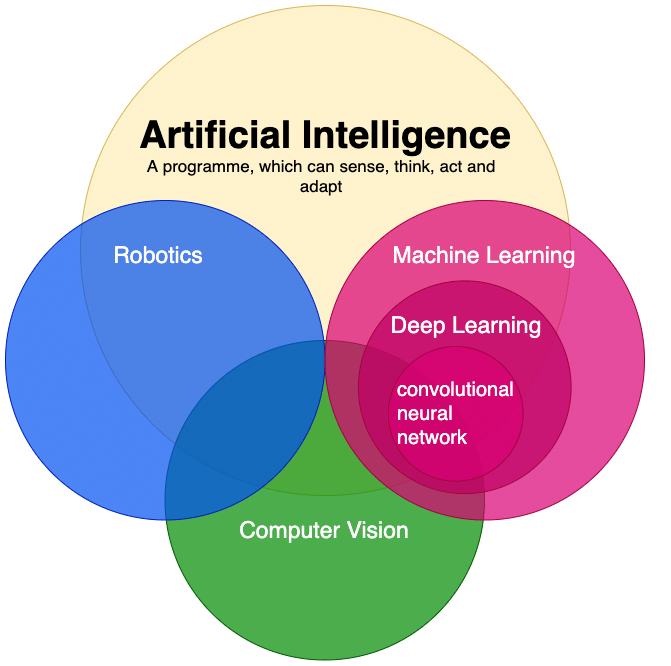
\includegraphics[width=\textwidth]{Figs/Ai1}
\resizebox{\columnwidth}{!}{%
				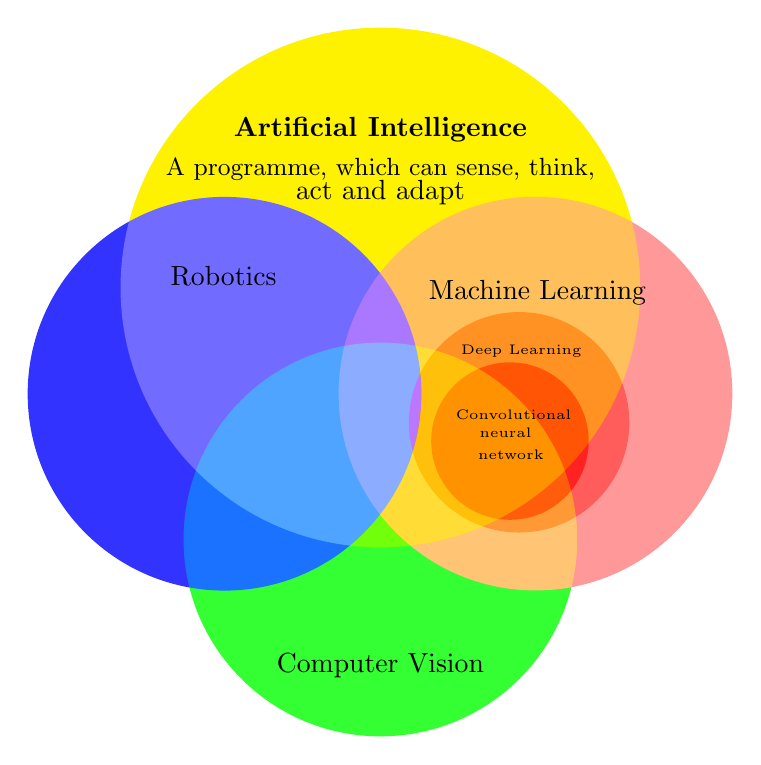
\begin{tikzpicture}
				  \begin{scope}[blend group = soft light]
					\fill[blue!80] (190:2.01) circle (2.5);
					\fill[red!40]  (350:2) circle (2.5);
					\fill[green!80]   ( -90:2.2) circle (2.5);
					\fill[red!100]  (338:1.9) circle (1.4);
					\fill[black!100]  (330:1.9) circle (1);
					\fill[yellow!100]   ( 90:1) circle (3.3);
				   
				   
				  \end{scope}
				  \node at ( 90:3)      {\textbf{Artificial Intelligence}};
				  \node at ( 90:2.5)    {\small A programme, which can sense, think,};
				  \node at ( 90:2.2)    {act and adapt};
				  \node at ( 150:2.3)   {Robotics};
				  \node at ( 385:2.2)   {Machine Learning};
				  \node at ( 366:1.8)   {\tiny Deep Learning};
				  \node at ( 340:1.8)   {\tiny Convolutional};
				  \node at ( 332:1.8)   {\tiny neural};
				  \node at ( 326:2.0)   {\tiny network};
				  \node at ( -90:3.8)   {Computer Vision};
				\end{tikzpicture}
}

			 \end{center}
		\end{column}
	\end{columns}

\end{frame}


%* Vision por Computadora

\begin{frame}{Visión por Computadora}
%\begin{block}{Fundamentación} 
\begin{columns}
\begin{column}{0.60\textwidth}
    \begin{center}
\begin{itemize}
\item La visión por computadora imita la percepción humana y las capacidades de razonamiento.
\item Se intenta inferir conocimiento a partir de imágenes o videos.
\item Procesamiento de imágenes es una fase temprana de la VC. La entrada es una imagen y la salida es otra imagen.
\item En la visión por computadora, la entrada es una imagen pero la salida son datos. 
\end{itemize}
     \end{center}

\end{column}
\begin{column}{0.40\textwidth}  
    \begin{center}
     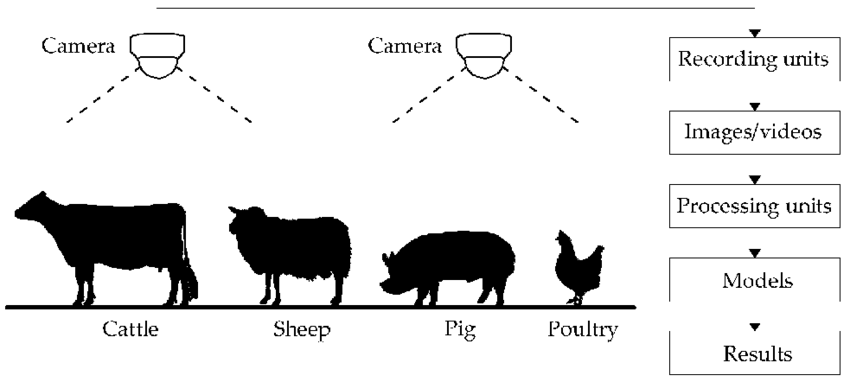
\includegraphics[width=0.9\textwidth]{Figs/VC}
     \end{center}
\end{column}
\end{columns}
%\end{block} 
\end{frame}

\begin{frame}{Visión por Computadora (Template Matching)}

Permite comparar imágenes aplicando operaciones de comparación entre regiones.
\begin{columns}
  \column {0.5\textwidth}
  \begin{itemize}
    \item Algoritmos clásicos basados en correlación: SAD, SSD, Rank.
	  \begin{itemize}
		    \item Ventajas: Facil de entender, rápidos
		    \item Desventajas: Sensibles a la escala, a rotaciones y a cambios en la iluminación. 
	  \end{itemize}
    \item Algoritmos modernos basados Aprendizaje Profundo
		\begin{itemize}
		    \item Ventajas: Buen desempeño 
		    \item Desventajas: Requieren de entrenamiento con muchas imágenes
	  \end{itemize}

  \end{itemize}
    \column {0.5\textwidth}  
        \begin{center}
            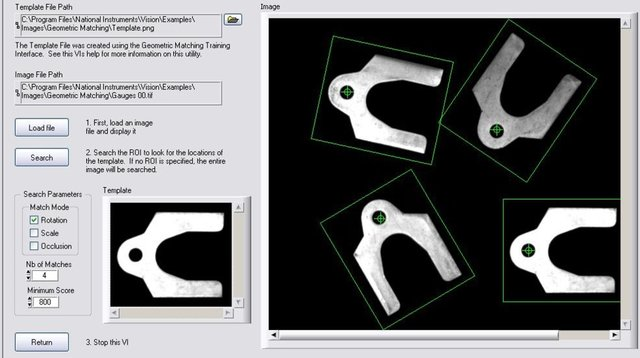
\includegraphics[width=\textwidth]{00_IntroComputerVision/figs/Industrial-software-example-for-Template-Matching_W640}\\
     \end{center}

    \end{columns}
\end{frame}



%* Graficos por Computadora

\begin{frame}{Gráficos por Computadora}
%\begin{block}{Gráficos por Computadora} 
\begin{columns}
\begin{column}{0.58\textwidth}
    \begin{center}

\begin{itemize}
\item Es la rama de las CC encargada de la producción de imágenes y animaciones empleadas en juegos de computadora y simulaciones, en algunos casos incluyendo elementos fotorealisticos.
\item Se requieren conocimientos de geometría, algebra, cálculo, física, programación (estructura de datos). 
\item Existen liberias de bajo nivel (OpenGL) hasta frameworks (Unity, Unreal).
\end{itemize}
     \end{center}

\end{column}
\begin{column}{0.42\textwidth}  
    \begin{center}
     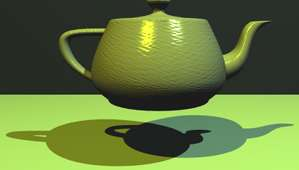
\includegraphics[width=0.9\textwidth]{Figs/GC1}\\
     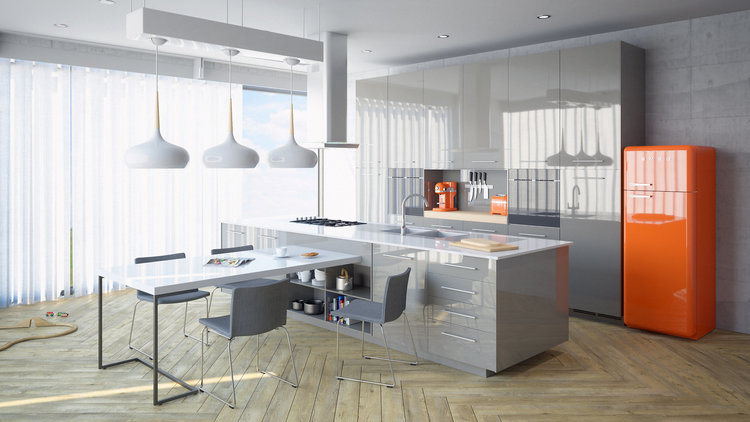
\includegraphics[width=0.9\textwidth]{Figs/GC2}\\
     \end{center}
\end{column}
\end{columns}
%\end{block} 
\end{frame}


%* Realidad Virtual

\begin{frame}{Realidad Aumentada (AR) \footnotemark}
%\begin{block}{Realidad Aumentada (AR) \footnotemark} 
\begin{columns}
\begin{column}{0.49\textwidth}
\begin{itemize}
\item La AR es una experiencia que traslapa elementos digitales (modelados por computadora) con el mundo físico del usuario (adquirido mediante una cámara). 
\item Los elementos digitales se combinan con las vistas del mundo real.
\end{itemize}
\end{column}
\begin{column}{0.49\textwidth}
\begin{center}
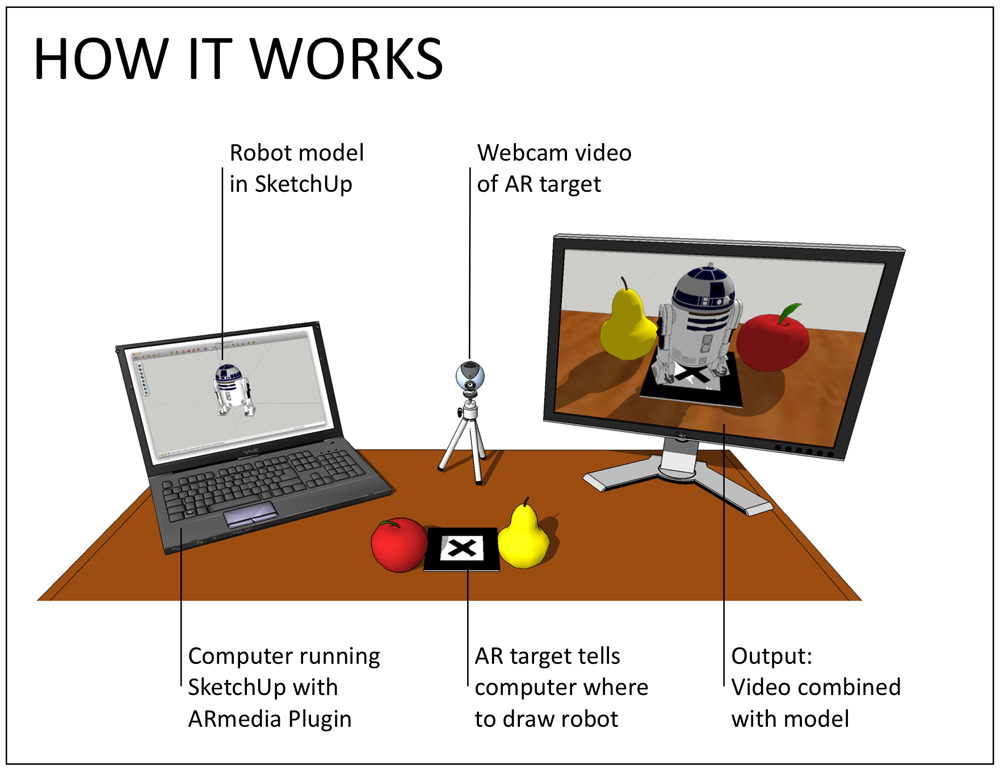
\includegraphics[width=0.95\textwidth]{Figs/AR_HowItWorks}
\end{center}
\end{column}
\end{columns}
\footnotetext{\url{http://photos1.blogger.com/img/m-a310d3b7b46f285189e1d6da63a1afd13be4ffc4.jpg}}
%\end{block} 
\end{frame}

\begin{frame}{Pasos en la detección de marcadores de AR \footnotemark}
%\begin{block}{Pasos en la detección de marcadores de AR \footnotemark} 
\begin{columns}
\begin{column}{0.39\textwidth}
\begin{enumerate}
\item Umbralización.
\item Detección del Marcador.
\item Estimación de Pose y Posición.
\item Empalme del modelo 3D.
\end{enumerate}
\end{column}
\begin{column}{0.59\textwidth}
\begin{center}
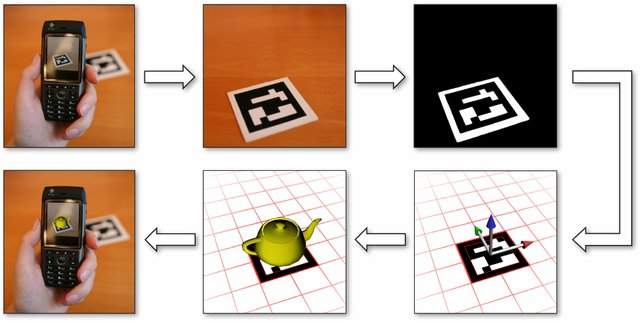
\includegraphics[width=0.95\textwidth]{Figs/AR_WorkFlow}
\end{center}
\end{column}
\end{columns}
%\end{block} 
\footnotetext{\fullcite{Wagner_ArToolKitPlus2007}}
\end{frame}


\begin{frame}{Tipos de Aplicación de AR \footnotemark}
%\begin{block}{Tipos de Aplicación de AR \footnotemark} 
\begin{columns}
\begin{column}{0.98\textwidth}
    \begin{center}

\begin{itemize}
\item Basadas en Localización. Están basada en sensores GPS para determinar la ubicación del dispositivo para crear objetos AR
\item Basadas en Visión – Utilizan una cámara, aunque también es posible incorporar sensores (compass, acelerómetros, giroscopios, etc). 
\begin{itemize}
\item  Requieren Marcadores (Marker) – Localizan un patrón o marcador QR  y renderizan un objeto 3D basado en su localización en el espacio real. 
\item  No requieren marcadores (Markerless)– Se emplean esquinas y puntos característicos del espacio real
\end{itemize}
\end{itemize}
     \end{center}

\end{column}
\end{columns}
%\end{block} 
\footnotetext{\url{https://fswa-net.com/index.php/news/use-of-ar-technology}}

%\\setcounter{footnote}{0}
\end{frame}


\begin{frame}{Aplicaciones de RA}
%\begin{block}{Aplicaciones de RA} 
\begin{itemize}
\item Aplicaciones principales: Arquitectura, Cosméticos, Contenido social, Marketing, Juegos, etc
\end{itemize}

\begin{columns}
\begin{column}{0.49\textwidth}
\begin{itemize}
\item Houzz
\end{itemize}
\begin{center}
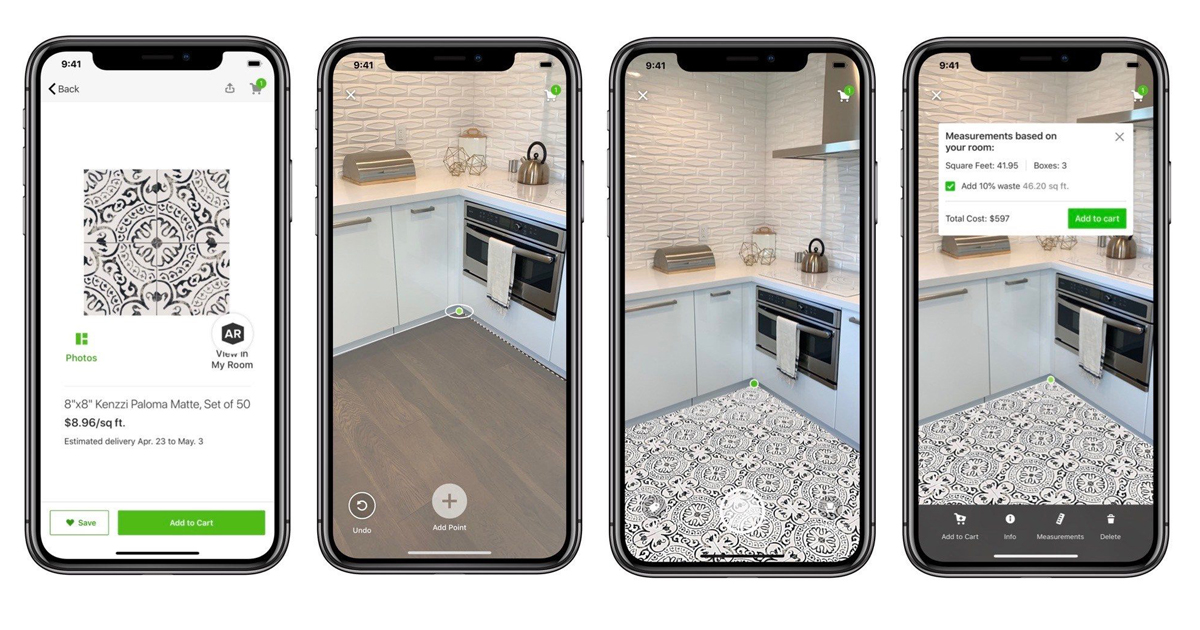
\includegraphics[width=0.9\textwidth]{Figs/AR_App}\\
\end{center}
\end{column}
\begin{column}{0.49\textwidth}  

\begin{itemize}
\item Pokemon Go
\end{itemize}
    \begin{center}
     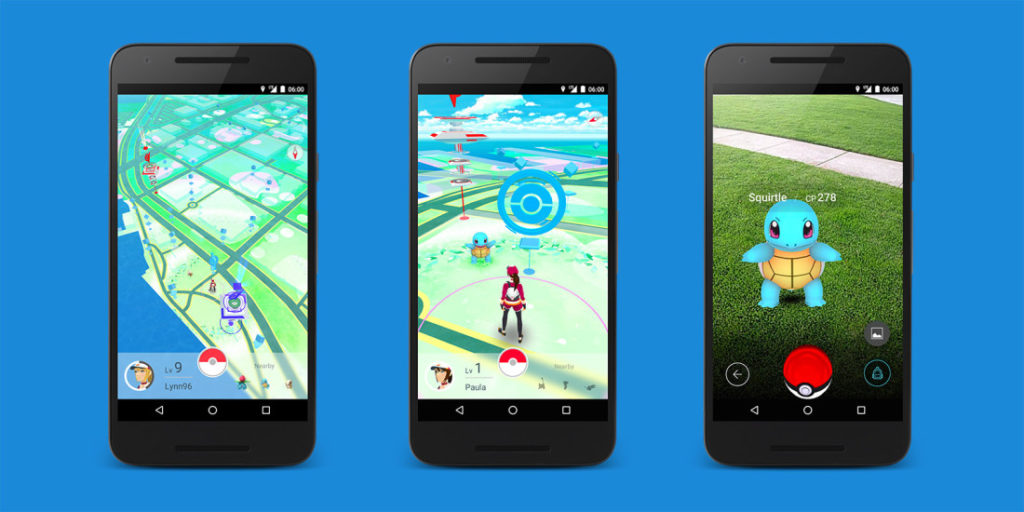
\includegraphics[width=0.9\textwidth]{Figs/Pokemon}
     \end{center}
\end{column}
\end{columns}
%\end{block} 
\end{frame}


\begin{frame}{Realidad Virtual - Antecedente hist\'orico}

\begin{columns}
\begin{column}{0.49\textwidth}


\begin{itemize}
\item Un estereoscopio proporciona im\'agenes separadas para cada ojo mediante lentes individuales, donde cada imagen tiene una variante en el angulo de captura y un desplazamiento horizontal.
\item El cerebro de una persona con una percepción binocular normal de la profundidad al utilizar el estereoscopio ``mezcla'' ambas imagenes para crear una  ``ventana estereoscópica''
\end{itemize}
\end{column}

\begin{column}{0.49\textwidth}

\begin{center}
	\begin{tabular}{cc}
        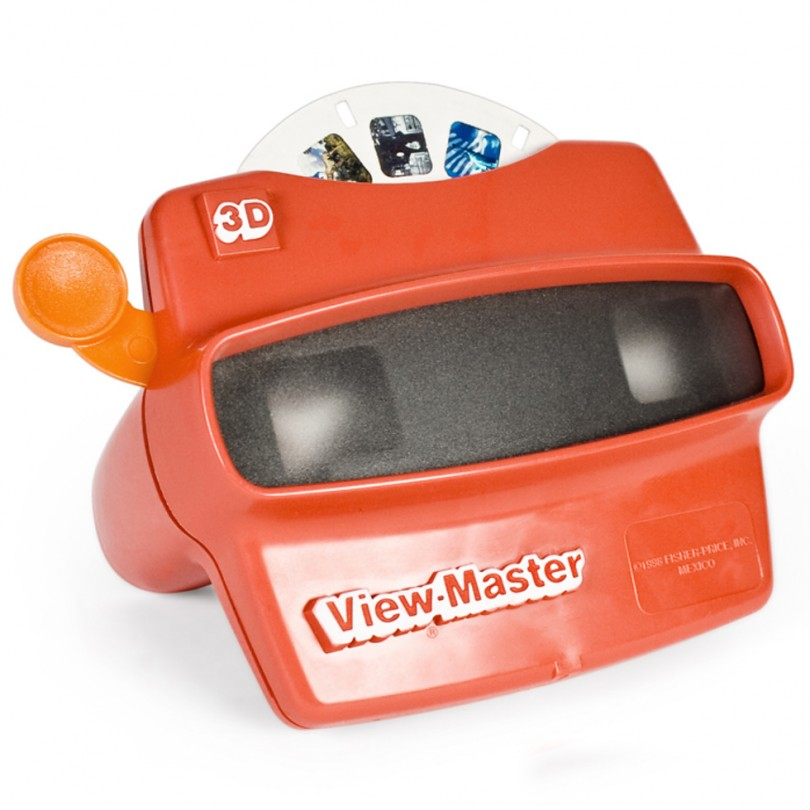
\includegraphics[width=0.45\linewidth]{Figs/view_master_blog-810x810.jpg} &
		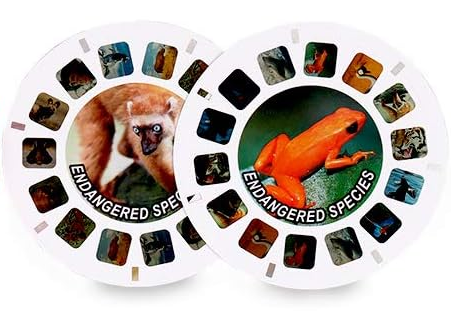
\includegraphics[width=0.45\linewidth]{Figs/DiscosViewMaster.png}    
	\end{tabular}

	\begin{tabular}{cc}
	\centering
        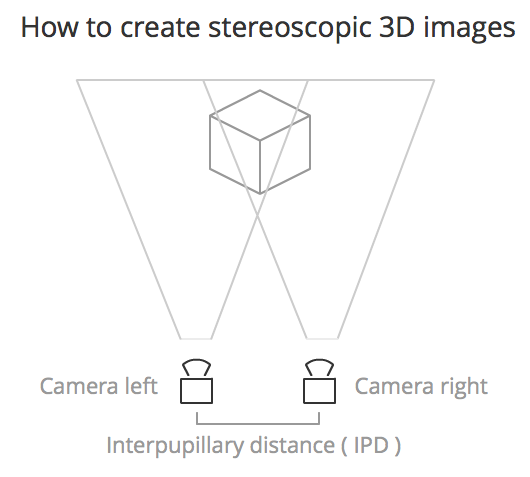
\includegraphics[width=0.49\linewidth]{Figs/VirtualReal1} &
        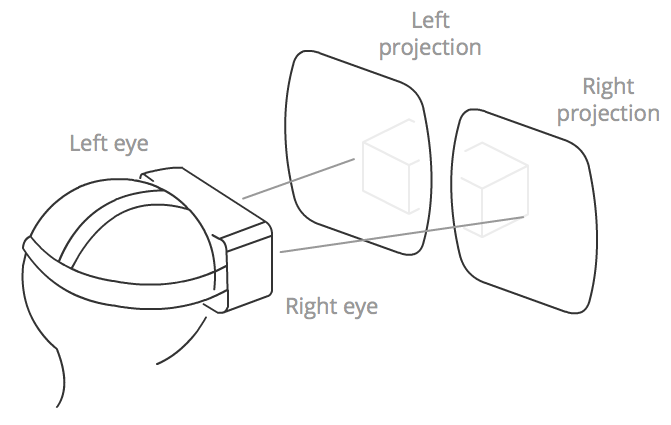
\includegraphics[width=0.49\linewidth]{Figs/VirtualReal2} \\

	\end{tabular}
\end{center}
\end{column}

\end{columns}

\end{frame}




\begin{frame}{Realidad Virtual (VR)}
%\begin{block}{Realidad Virtual (VR)} 
		\begin{itemize}
			\item La Realidad virtual (RV) emplea modelos y simulaciones por computadora que permite a una persona interactuar con un entorno visual artificial tridimensional (3D)
			\item En un formato típico de RV, un usuario lleva un casco con una pantalla estereoscópica para ver imágenes animadas de un entorno simulado
			\item El dispositivo m\'as econ\'omico para aplicaciones de RV es un tel\'efono inteligente 
		\end{itemize}
    \begin{center}
	\begin{tabular}{ccc}
    	\centering
		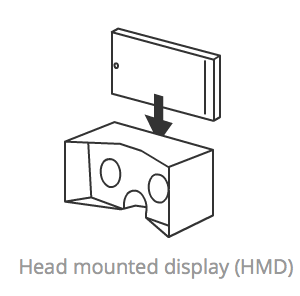
\includegraphics[width=0.25\linewidth]{Figs/MobileVR2} & 
        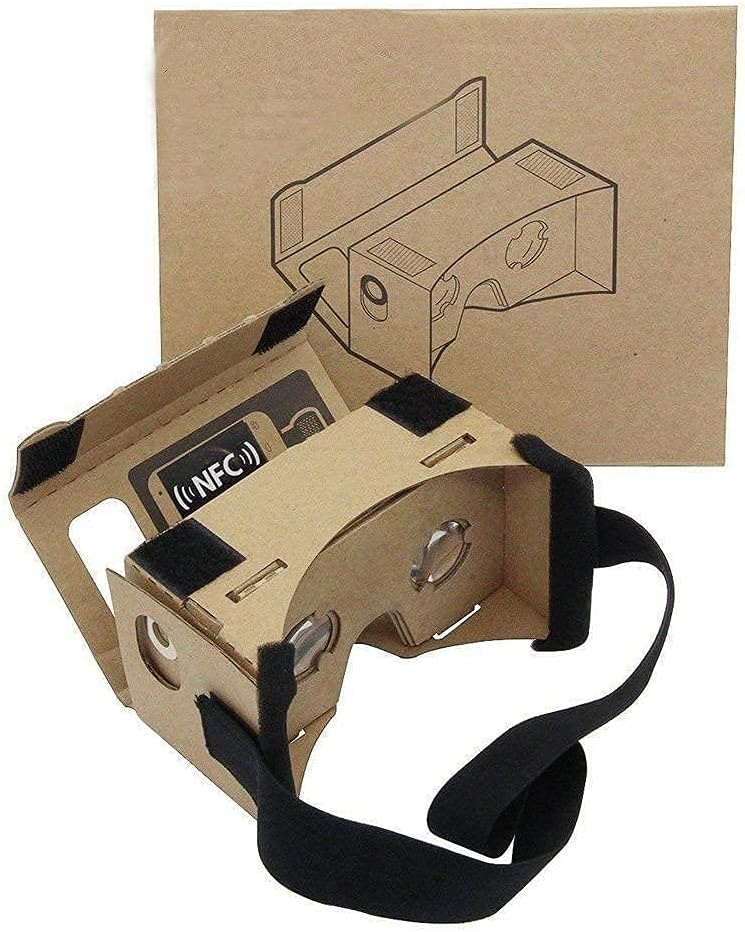
\includegraphics[width=0.19\linewidth]{Figs/CardBoard} & 		
        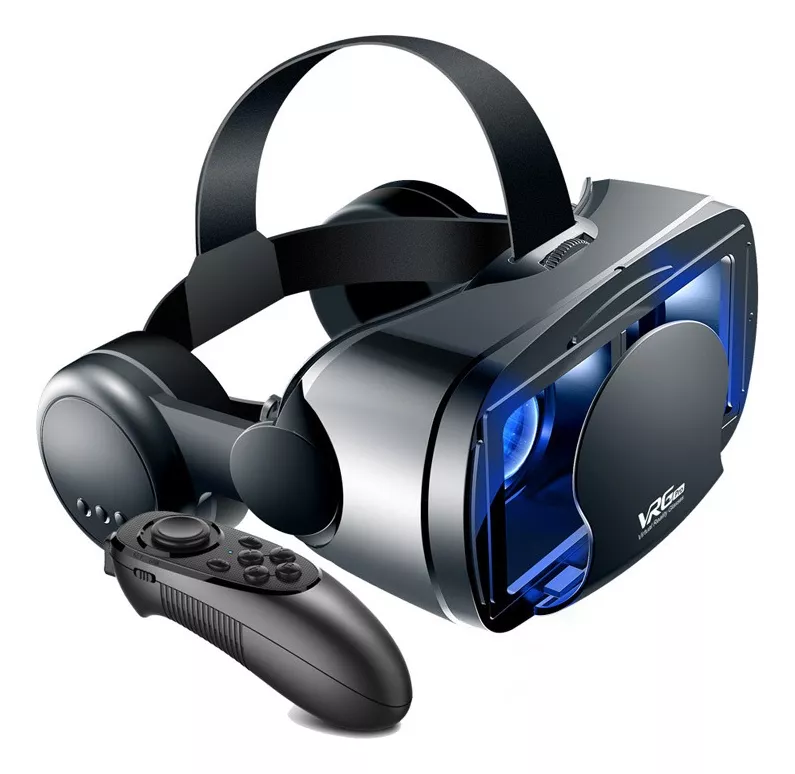
\includegraphics[width=0.19\linewidth]{Figs/VRGPro} 		
	\end{tabular}
		 \end{center}
%\end{block} 
\footnotetext{\url{https://reference.codeproject.com/book/dom/webvr_api/webvr_concepts}}
\end{frame}


\begin{frame}{Costos de Dispostivos HeadSets para VR}
\begin{columns}
\begin{column}{0.49\textwidth}
\begin{itemize}
\item Meta Quest 3 (499 USD)
\item Sony PlayStation VR2 (599 USD)
\item Meta Quest Pro (900 USD)
\item Valve Index VR Kit (1350 USD)
\item HTC Vive Pro 2 (1400 USD)
\end{itemize}

\begin{center}
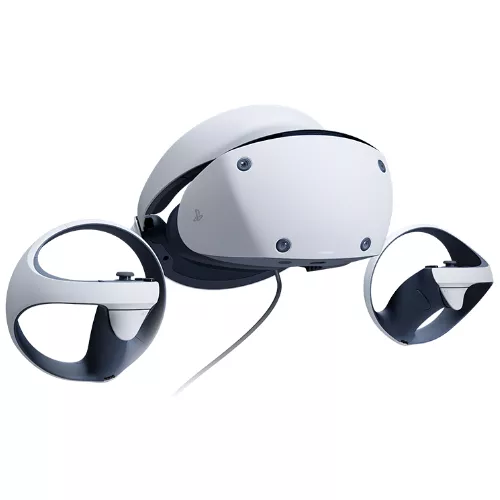
\includegraphics[width=0.75\textwidth]{Figs/sony.png}
\end{center}
\end{column}
\begin{column}{0.49\textwidth}
\begin{center}
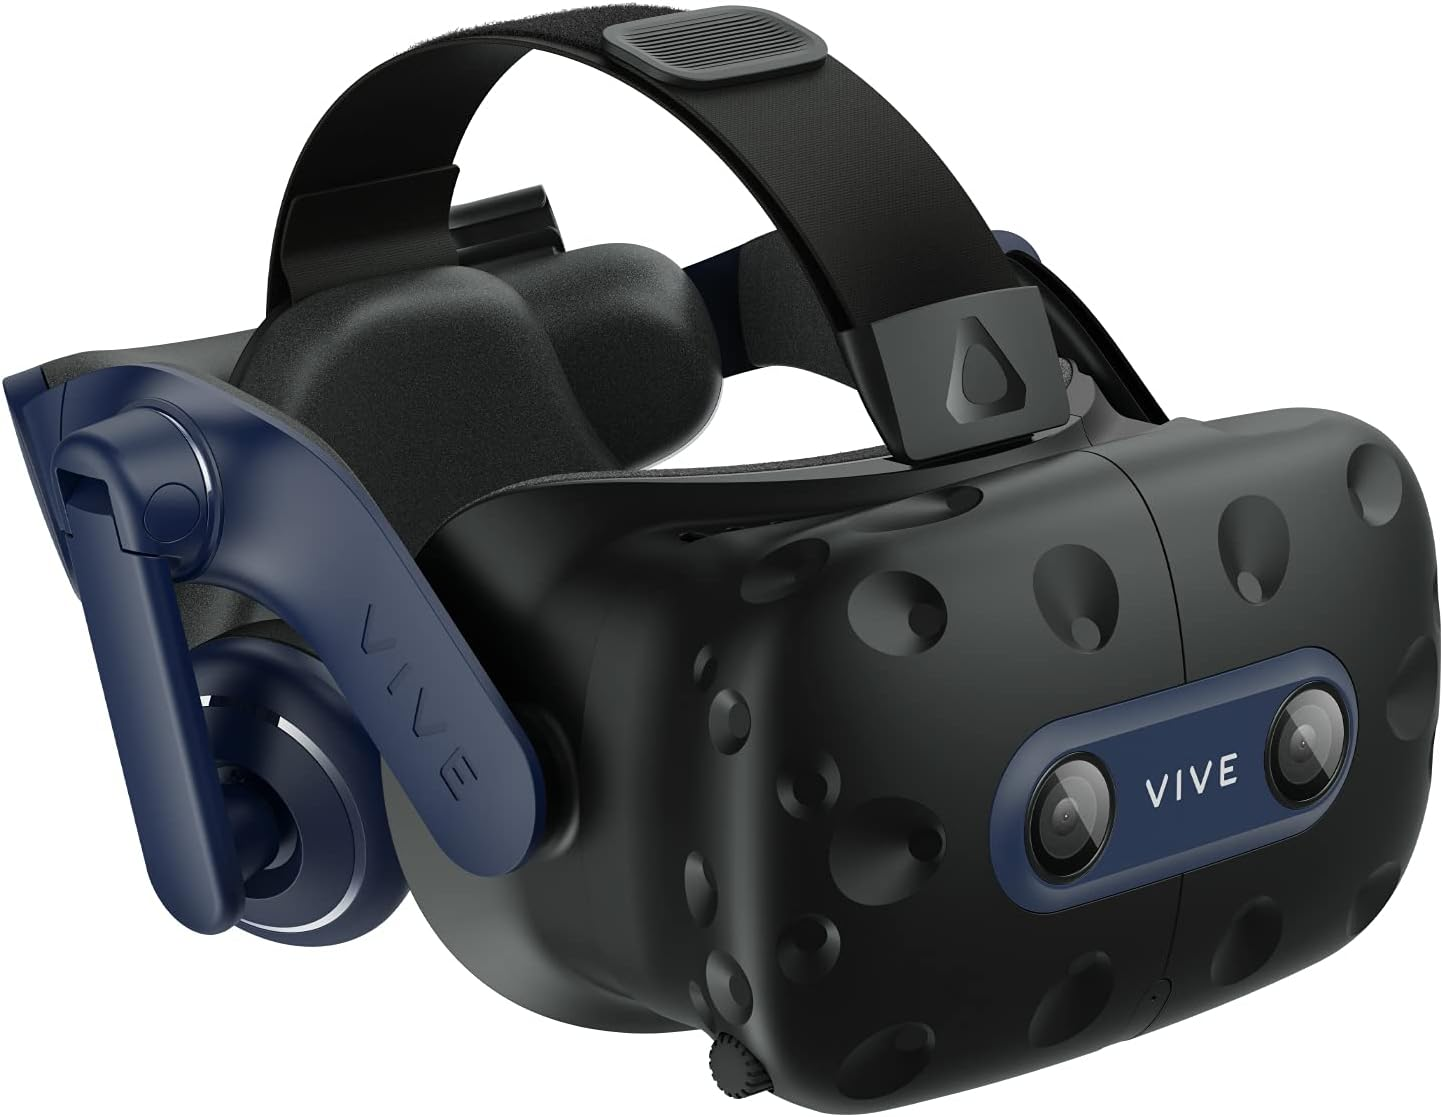
\includegraphics[width=0.75\textwidth]{Figs/HTC.jpg}\\
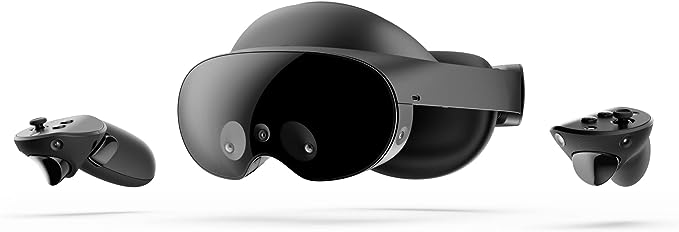
\includegraphics[width=0.95\textwidth]{Figs/MetaPro.jpg}
\end{center}
\end{column}
\end{columns}
\end{frame}


\begin{frame}{Relación entre RA/RV - Teléfonos Inteligentes}
Los teléfonos inteligentes son una de las principales plataformas para sistemas de \textbf{realidad aumentada (AR) y realidad virtual (VR)}:  
\begin{itemize}
\item Tienen hardware avanzado (cámaras, sensores de movimiento, procesadores gráficos) que permiten ejecutar experiencias inmersivas de AR y VR sin necesidad de equipos especializados.  
\item Existen accesorios como **gafas VR para móviles** (ej. Google Cardboard, Samsung Gear VR) que convierten un teléfono en un visor de realidad virtual.  
\item Existen herramientas para crear apps de RA y RV
\item Muchas aplicaciones combinan AR con inteligencia artificial para ofrecer experiencias interactivas y personalizadas.  
\item Gran cantidad de aplicaciones prácticas
\end{itemize}
\end{frame}

%* Realidad Aumentada
%Parte 2: Intro a Telefonos Moviles
\section[Tools]{Herramientas}
%* Android y SO para smartphones
%
\begin{frame}{Programación Móvil}
%\begin{block}{Programación Móvil} 
\begin{columns}
\begin{column}{0.98\textwidth}
    \begin{center}

\begin{itemize}
\item Es la actividad de desarrollar una aplicación específicamente para teléfonos inteligentes.
\item Estas aplicaciones se encuentran preinstaladas en el teléfono o pueden ser instaladas por el usuario mediante una tienda de aplicaciones (App Store o Google Play)
\item Las tareas que tradicionalmente hacíamos en la PC ahora están migrando hacia el teléfono inteligente
\item Principales sistemas operativos móviles: Android, iOS,
\item Enfocados principalmente en el desarrollo de aplicaciones NATIVAS.
\item Lenguajes de programación: Java, Kotlin.
\end{itemize}
     \end{center}

\end{column}
\end{columns}
%\end{block} 
\end{frame}


\begin{frame}
\frametitle{Codificacion de un algoritmo en varios lenguajes de programaci\'on (Python - Kotlin)} 
\begin{columns}
\column{0.45\linewidth}
\begin{block}{Codificacion del Algoritmo en Python}
\inputminted[linenos,fontsize=\tiny]{python}{00_IntroProgramacionYMoviles/Hello.py}
\end{block}
\column{0.45\linewidth}
\begin{block}{Codificacion del Algoritmo en Kotlin}
\inputminted[linenos,fontsize=\tiny]{python}{00_IntroProgramacionYMoviles/Hello.kt}
\end{block}
\end{columns}
\end{frame}



\begin{frame}
\frametitle{Sistema Operativo}  
\begin{columns}
%\column{0.32\linewidth}
\column{0.65\linewidth}
\begin{block}{}
Un Sistema Operativo (SO) es un programa (software) que al arrancar la computadora** se encarga de gestionar todos los recursos del sistema informático permitiendo así la comunicación entre el usuario y la computadora. 
\end{block}
\begin{center}
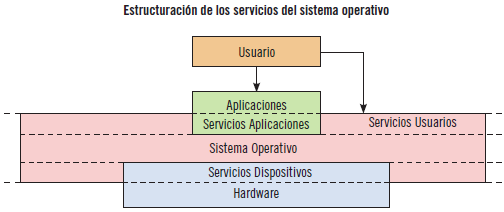
\includegraphics[width=0.95\linewidth]{00_IntroProgramacionYMoviles/SistemaOperativo1.png} 
\end{center}
\tiny{\url{https://reader.digitalbooks.pro/content/preview/books/38230/book/OEBPS/Text/c1.html}}

\column{0.32\linewidth}
\begin{center}
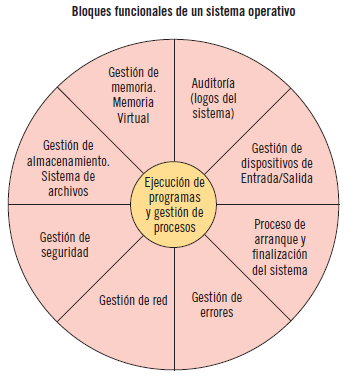
\includegraphics[width=0.95\linewidth]{00_IntroProgramacionYMoviles/SistemaOperativo2.png} 
\end{center}
\end{columns}

\end{frame}


\begin{frame}
\frametitle{Sistemas Operativos para PCs}  

\begin{columns}
\column{0.32\linewidth}
\begin{center}

\includegraphics[width=0.95\linewidth]{00_IntroProgramacionYMoviles/Windows11.png} 
\end{center}

\column{0.32\linewidth}
\begin{center}
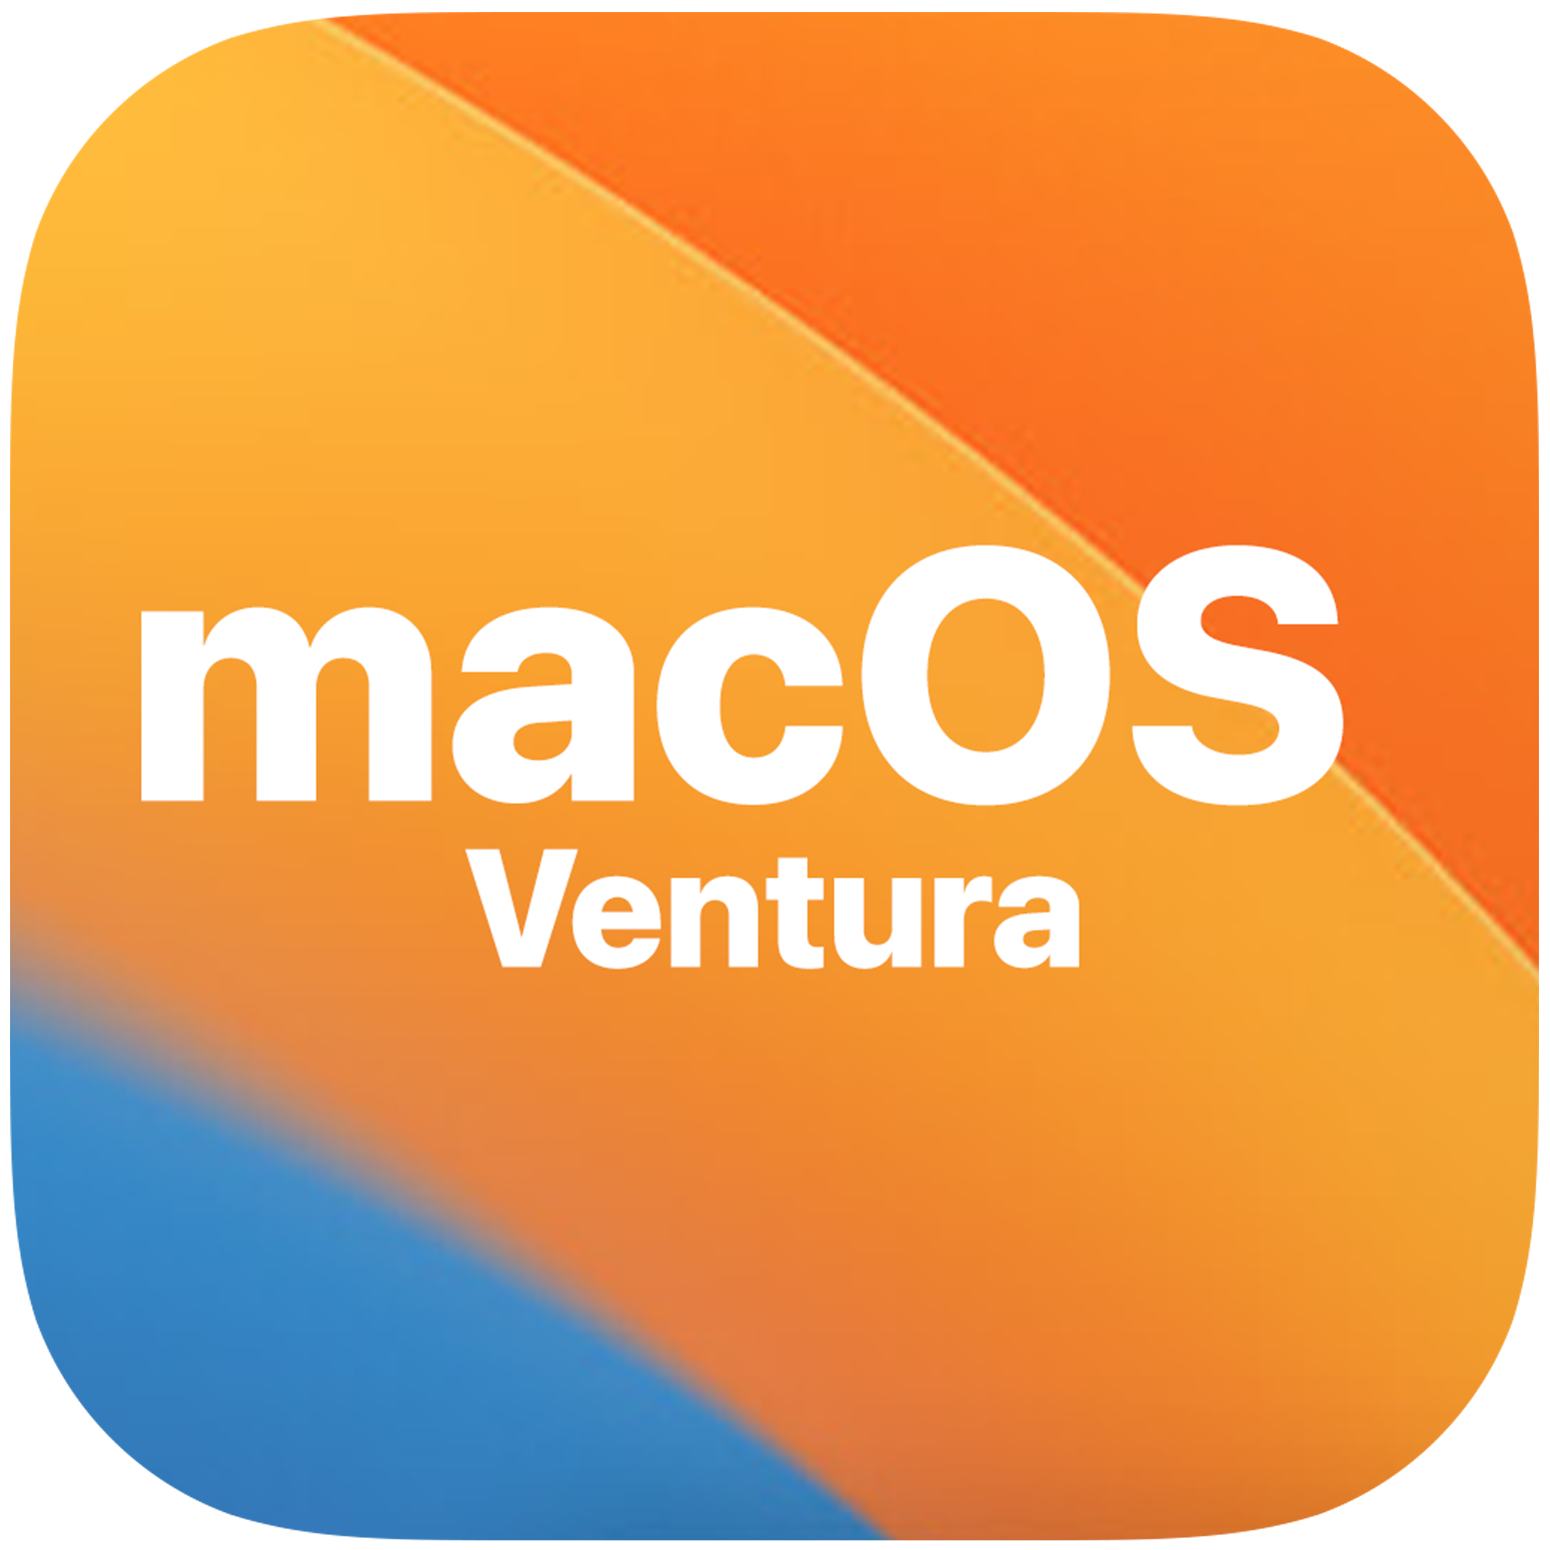
\includegraphics[width=0.95\linewidth]{00_IntroProgramacionYMoviles/MacOS.png} 
\end{center}

\column{0.32\linewidth}
\begin{center}

\includegraphics[width=0.95\linewidth]{00_IntroProgramacionYMoviles/Linux.png} 
\end{center}
\end{columns}

\end{frame}





\begin{frame}
\frametitle{Telefono Celular No-inteligente vs Telefono Celular Inteligente}  

\begin{columns}
\column{0.46\linewidth}
\begin{block}{Tel\'efono No-inteligente}
\begin{itemize}
\item Su funcionalidad principal era la comunicaci\'on (llamadas o mensajes) a trav\'es de la red celular (GSM)
\end{itemize}
\end{block}
\begin{block}{Tel\'efono inteligente}
\begin{itemize}
\item Interfaz de entrada: Pantalla Touch (a color, de alta definici\'on) 
\item Conexi\'on a Internet: WiFi, GSM (4G o 5G)
\item Comunicaci\'on con otros dispositivos: Bluetooth, NFC
\item C\'amaras (Frontal y Posterior)
\end{itemize}
\end{block}

\column{0.18\linewidth}
\begin{center}
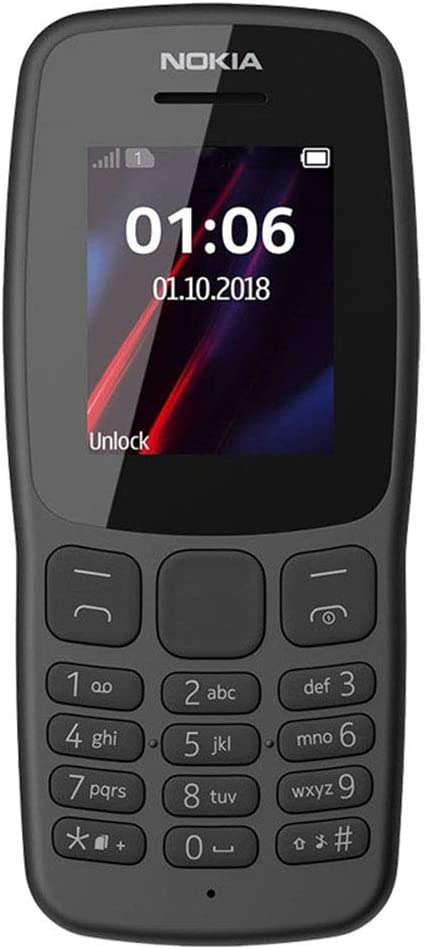
\includegraphics[width=0.95\linewidth]{00_IntroProgramacionYMoviles/FeaturePhone_Nokia.png} 
\end{center}
\column{0.28\linewidth}
\begin{center}
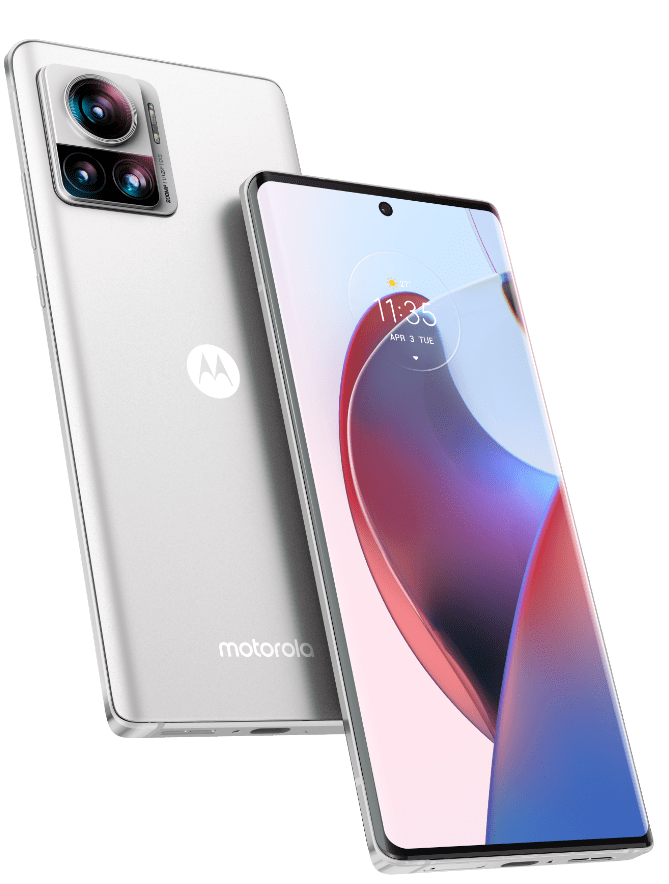
\includegraphics[width=0.95\linewidth]{00_IntroProgramacionYMoviles/Smartphone_Motorola.png} 
\end{center}
\end{columns}
\end{frame}

\begin{frame}
\frametitle{Sistemas Operativos para Telefonos Inteligentes} 
\begin{columns}
\column{0.32\linewidth}
\begin{center}

\includegraphics[width=0.95\linewidth]{00_IntroProgramacionYMoviles/Android.png} 
\end{center}

\column{0.32\linewidth}
\begin{center}

\includegraphics[width=0.95\linewidth]{00_IntroProgramacionYMoviles/iOs.png} 
\end{center}

\column{0.32\linewidth}
\begin{center}

\includegraphics[width=0.95\linewidth]{00_IntroProgramacionYMoviles/WindowsPhone.png} 
\end{center}
\end{columns}
 
\end{frame}


\begin{frame}
\frametitle{Android} 
\begin{columns}
\column{0.64\linewidth}
\begin{itemize}
\item Android es un sistema operativo móvil basado en Linux 
\item Principalmente orientado a dispositivos de pantalla t\'actil (Smartphone, tablets, smartwatches, etc)
\item Fue desarrollado por Android Inc (Adquirida por Google en 2005)
\item Vinculado con un grupo de empresas (HTC, Sony, Motorola, Samsung, LG, Lenovo, entre otras) para la creaci\'on de un SO com\'un para sus dispositivos
\item A la fecha (Q1 2023), los tel\'efonos con SO Android concentran mas del 70\% del mercado global. 
\end{itemize}
\column{0.32\linewidth}
\begin{center}
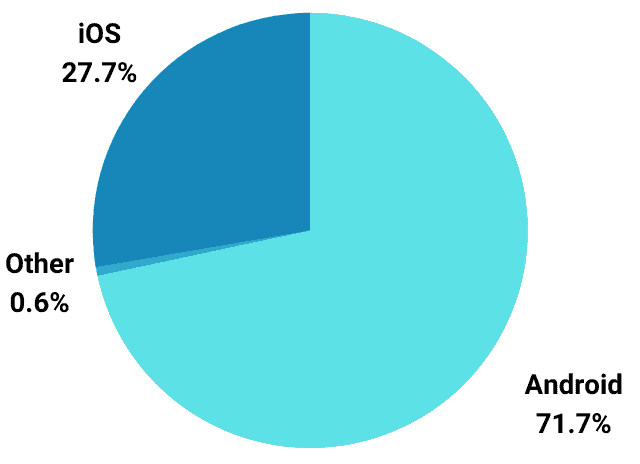
\includegraphics[width=0.95\linewidth]{00_IntroProgramacionYMoviles/AndroidVSIOs_WorldWide.png} 
\end{center}
\end{columns}
 
\end{frame}





\begin{frame}
\frametitle{Aplicaciones Móviles}  
\begin{columns}
\column{0.4\linewidth}
\begin{itemize}
\item Ejecutadas en el tel\'efono
\item La entrada de datos es mediante un teclado ``virtual''
\item El apuntador del raton es la pantalla 
\item Incluyen una interfaz de usuario gr\'afica (GUI) 
\item Es posible descargar miles de \'estas en nuestros dispositivos
\end{itemize}
\column{0.30\linewidth}
\begin{center}
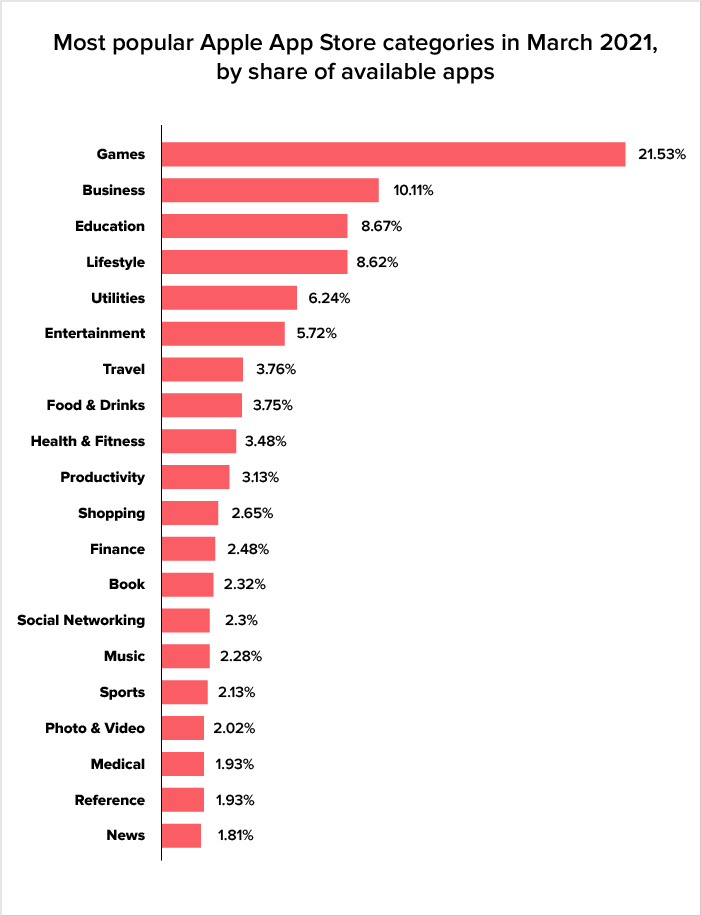
\includegraphics[width=0.95\linewidth]{00_IntroProgramacionYMoviles/TiposAplicaciones.png} 
\end{center}
\column{0.30\linewidth}
\begin{center}
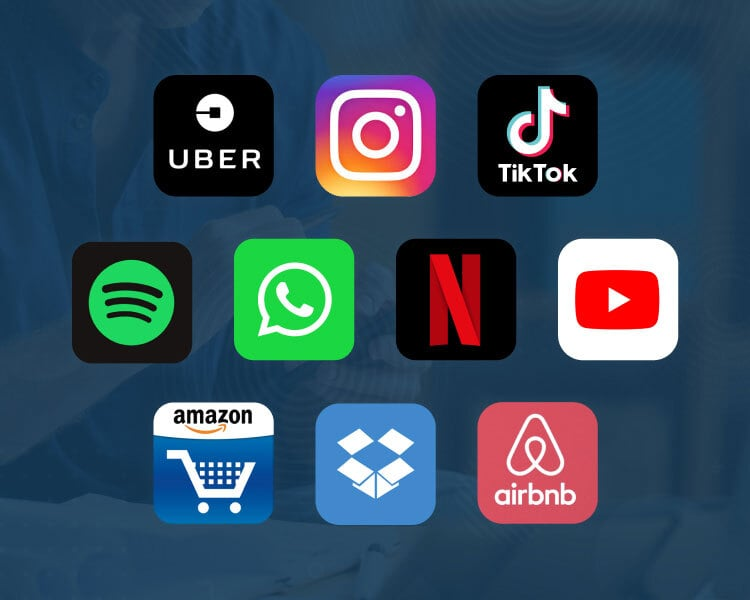
\includegraphics[width=0.95\linewidth]{00_IntroProgramacionYMoviles/most-popular-apps.jpg} 
\tiny{\url{https://www.netsolutions.com/insights/top-10-most-popular-apps-2018/}}  
\end{center}
\end{columns}
\end{frame}


\begin{frame}
\frametitle{Android Studio}  

\begin{itemize}
\item Android Studio es un entorno oficial de desarrollo integrado (IDE) para el sistema operativo Android de Google
\item La primera versi\'on se libera en el año 2013, siendo el lenguaje de programacion Java
\item En 2019, se reemplaza el lenguaje oficial de desarrollo por Kotlin, aunque Java todav\'ia es soportado
\item Es gratis, se puede descargar e instalar en cualquier computadora sin importar el sistema operativo (Windows, Linux y MacOS)
\url{https://developer.android.com}
\end{itemize}
\end{frame}

%* Tomada del Taller del CBTIS

\section[PyTI]{Programaci\'on y Tel\'efonos Inteligentes}

\section{Introducci\'on}

\begin{frame}
\frametitle{Computadora y Programabilidad}  
\begin{block}{Computadora}
Es una m\'aquina (electr\'onica) programable* que recibe y procesa datos para convertirlos en informaci\'on \'util. Contiene perif\'ericos de entrada (para introducir datos) y salida (para mostrar resultados) \pause
\end{block}
\begin{block}{Algoritmo}
Conjunto finito de instrucciones para resolver una tarea espec\'ifica \pause
\end{block}

\begin{block}{Programaci\'on}
El proceso de crear un software utilizando un lenguaje de programacion (C, C++, Java, Python, Kotlin, etc) \pause
\end{block}

\begin{block}{Programa}
Un conjunto de instrucciones que una computadora interpreta en una secuencia logica para llevar a cabo una tarea en particular \pause
\end{block}

\end{frame}

\begin{frame}
\frametitle{Diagrama de Flujo} 
\begin{columns}
\column{0.5\linewidth}
Un diagrama de flujo es una representaci\'on gr\'afica de un algoritmo, los pasos que los componen y la secuencia de ejecuci\'on de sus instrucciones
\begin{block}{Algoritmo}
Dise\~nar un algoritmo para comparar dos numeros
\end{block}

\column{0.5\linewidth}
\begin{center}
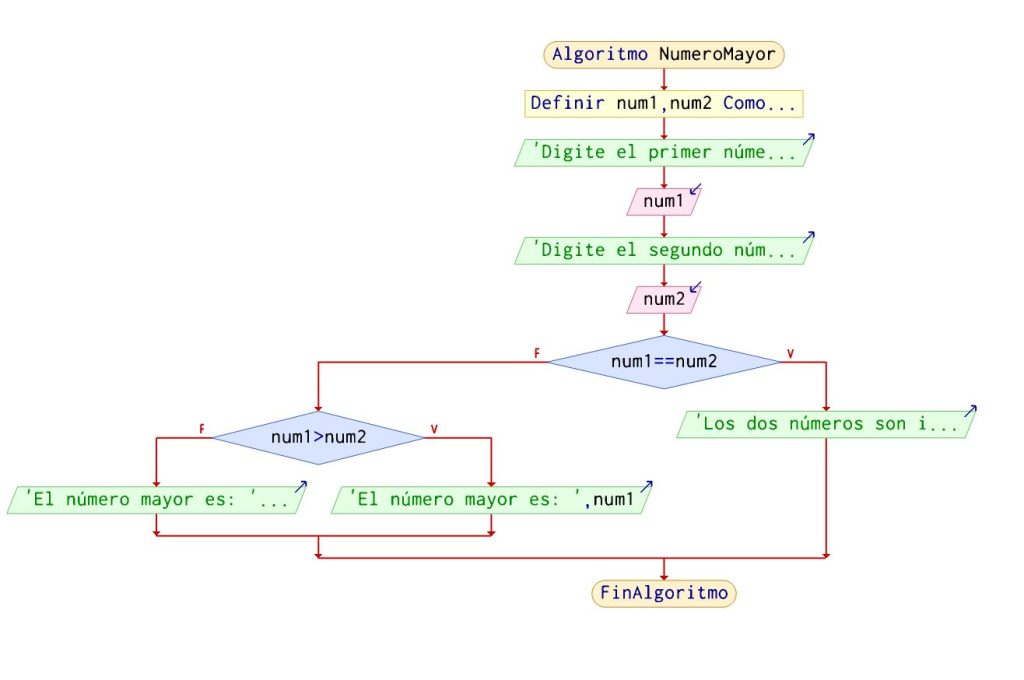
\includegraphics[width=0.95\linewidth]{00_IntroProgramacionYMoviles/DiagramaFlujo1.jpg} 
\end{center}
\end{columns}
\end{frame}

\begin{frame}
\frametitle{Codificacion de un algoritmo en varios lenguajes de programaci\'on (Python - Kotlin)} 
\begin{columns}
\column{0.45\linewidth}
\begin{block}{Codificacion del Algoritmo en Python}
\inputminted[linenos,fontsize=\tiny]{python}{00_IntroProgramacionYMoviles/Hello.py}
\end{block}
\column{0.45\linewidth}
\begin{block}{Codificacion del Algoritmo en Kotlin}
\inputminted[linenos,fontsize=\tiny]{python}{00_IntroProgramacionYMoviles/Hello.kt}
\end{block}
\end{columns}
\end{frame}



\begin{frame}
\frametitle{Sistema Operativo}  
\begin{columns}
%\column{0.32\linewidth}
\column{0.65\linewidth}
\begin{block}{}
Un Sistema Operativo (SO) es un programa (software) que al arrancar la computadora** se encarga de gestionar todos los recursos del sistema informático permitiendo así la comunicación entre el usuario y la computadora. 
\end{block}
\begin{center}
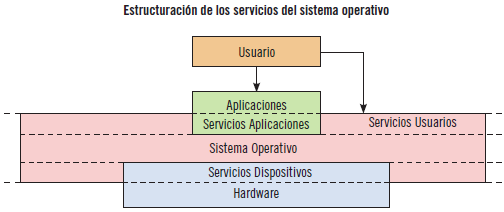
\includegraphics[width=0.95\linewidth]{00_IntroProgramacionYMoviles/SistemaOperativo1.png} 
\end{center}
\tiny{\url{https://reader.digitalbooks.pro/content/preview/books/38230/book/OEBPS/Text/c1.html}}

\column{0.32\linewidth}
\begin{center}
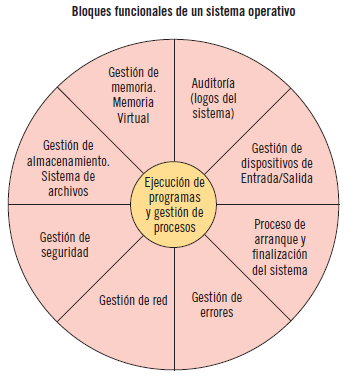
\includegraphics[width=0.95\linewidth]{00_IntroProgramacionYMoviles/SistemaOperativo2.png} 
\end{center}
\end{columns}

\end{frame}


\begin{frame}
\frametitle{Sistemas Operativos para PCs}  

\begin{columns}
\column{0.32\linewidth}
\begin{center}

\includegraphics[width=0.95\linewidth]{00_IntroProgramacionYMoviles/Windows11.png} 
\end{center}

\column{0.32\linewidth}
\begin{center}
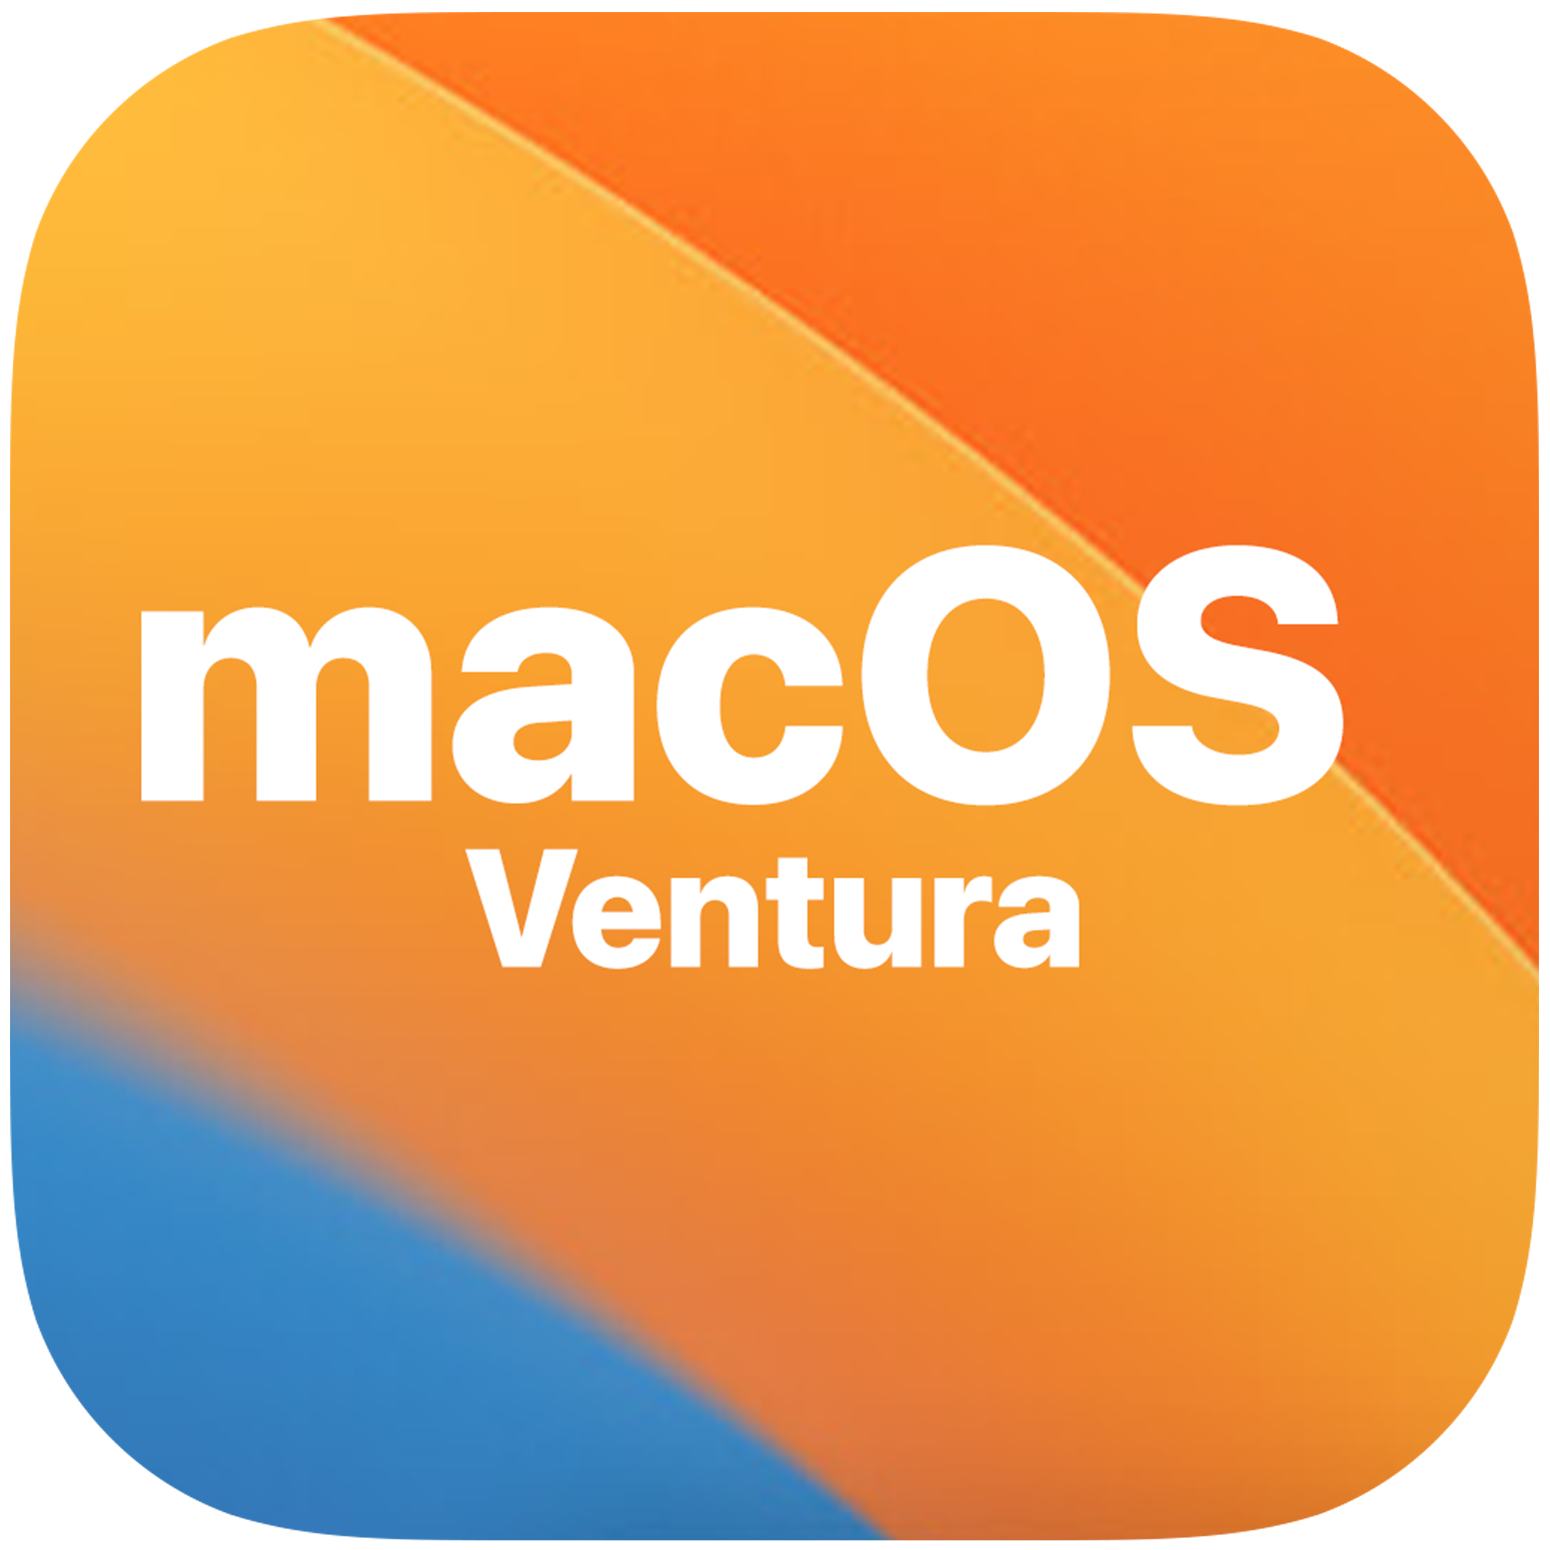
\includegraphics[width=0.95\linewidth]{00_IntroProgramacionYMoviles/MacOS.png} 
\end{center}

\column{0.32\linewidth}
\begin{center}

\includegraphics[width=0.95\linewidth]{00_IntroProgramacionYMoviles/Linux.png} 
\end{center}
\end{columns}

\end{frame}





\begin{frame}
\frametitle{Telefono Celular No-inteligente vs Telefono Celular Inteligente}  

\begin{columns}
\column{0.46\linewidth}
\begin{block}{Tel\'efono No-inteligente}
\begin{itemize}
\item Su funcionalidad principal era la comunicaci\'on (llamadas o mensajes) a trav\'es de la red celular (GSM)
\end{itemize}
\end{block}
\begin{block}{Tel\'efono inteligente}
\begin{itemize}
\item Interfaz de entrada: Pantalla Touch (a color, de alta definici\'on) 
\item Conexi\'on a Internet: WiFi, GSM (4G o 5G)
\item Comunicaci\'on con otros dispositivos: Bluetooth, NFC
\item C\'amaras (Frontal y Posterior)
\end{itemize}
\end{block}

\column{0.18\linewidth}
\begin{center}
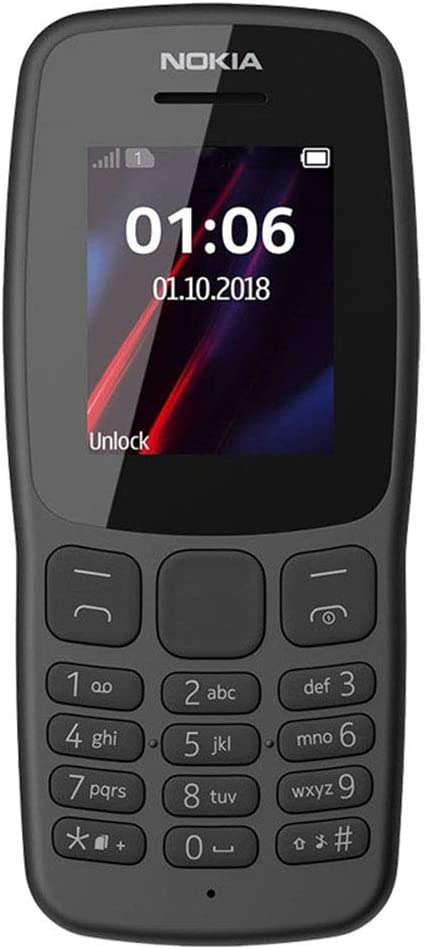
\includegraphics[width=0.95\linewidth]{00_IntroProgramacionYMoviles/FeaturePhone_Nokia.png} 
\end{center}
\column{0.28\linewidth}
\begin{center}
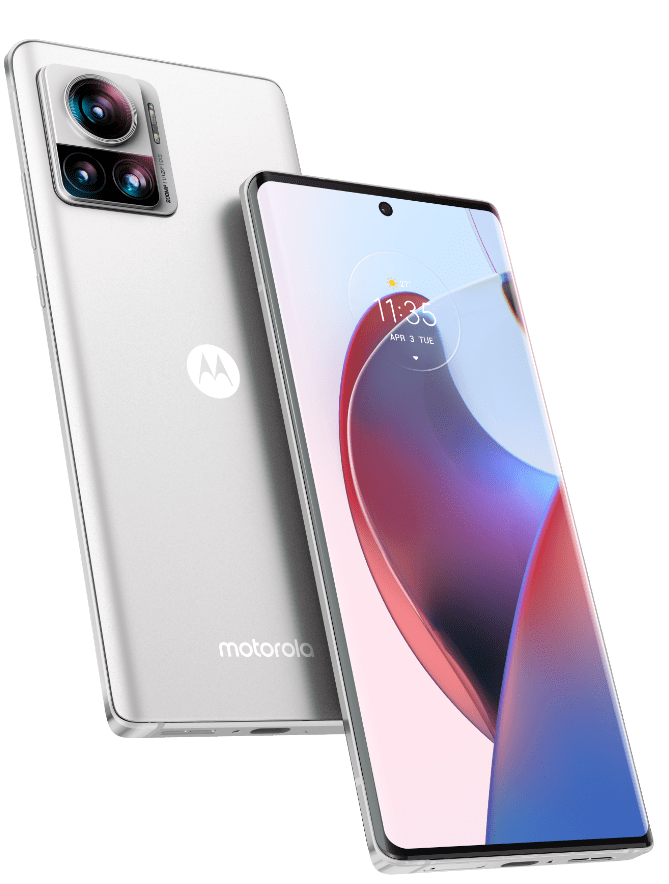
\includegraphics[width=0.95\linewidth]{00_IntroProgramacionYMoviles/Smartphone_Motorola.png} 
\end{center}
\end{columns}
\end{frame}

\begin{frame}
\frametitle{Sistemas Operativos para Telefonos Inteligentes} 
\begin{columns}
\column{0.32\linewidth}
\begin{center}

\includegraphics[width=0.95\linewidth]{00_IntroProgramacionYMoviles/Android.png} 
\end{center}

\column{0.32\linewidth}
\begin{center}

\includegraphics[width=0.95\linewidth]{00_IntroProgramacionYMoviles/iOs.png} 
\end{center}

\column{0.32\linewidth}
\begin{center}

\includegraphics[width=0.95\linewidth]{00_IntroProgramacionYMoviles/WindowsPhone.png} 
\end{center}
\end{columns}
 
\end{frame}


\begin{frame}
\frametitle{Android} 
\begin{columns}
\column{0.64\linewidth}
\begin{itemize}
\item Android es un sistema operativo móvil basado en Linux 
\item Principalmente orientado a dispositivos de pantalla t\'actil (Smartphone, tablets, smartwatches, etc)
\item Fue desarrollado por Android Inc (Adquirida por Google en 2005)
\item Vinculado con un grupo de empresas (HTC, Sony, Motorola, Samsung, LG, Lenovo, entre otras) para la creaci\'on de un SO com\'un para sus dispositivos
\item A la fecha (Q1 2023), los tel\'efonos con SO Android concentran mas del 70\% del mercado global. 
\end{itemize}
\column{0.32\linewidth}
\begin{center}
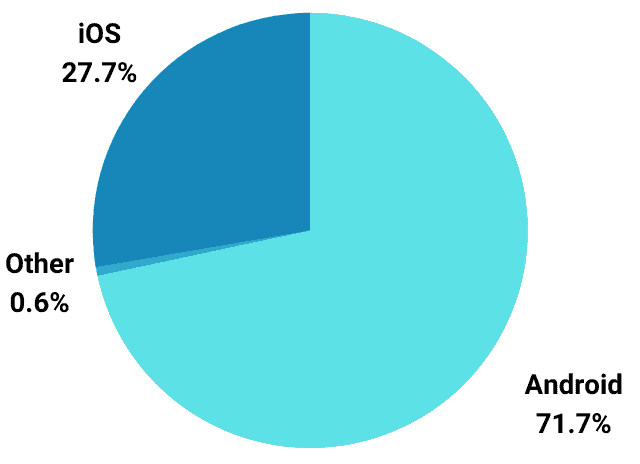
\includegraphics[width=0.95\linewidth]{00_IntroProgramacionYMoviles/AndroidVSIOs_WorldWide.png} 
\end{center}
\end{columns}
 
\end{frame}





\begin{frame}
\frametitle{Aplicaciones Móviles}  
\begin{columns}
\column{0.4\linewidth}
\begin{itemize}
\item Ejecutadas en el tel\'efono
\item La entrada de datos es mediante un teclado ``virtual''
\item El apuntador del raton es la pantalla 
\item Incluyen una interfaz de usuario gr\'afica (GUI) 
\item Es posible descargar miles de \'estas en nuestros dispositivos
\end{itemize}
\column{0.30\linewidth}
\begin{center}
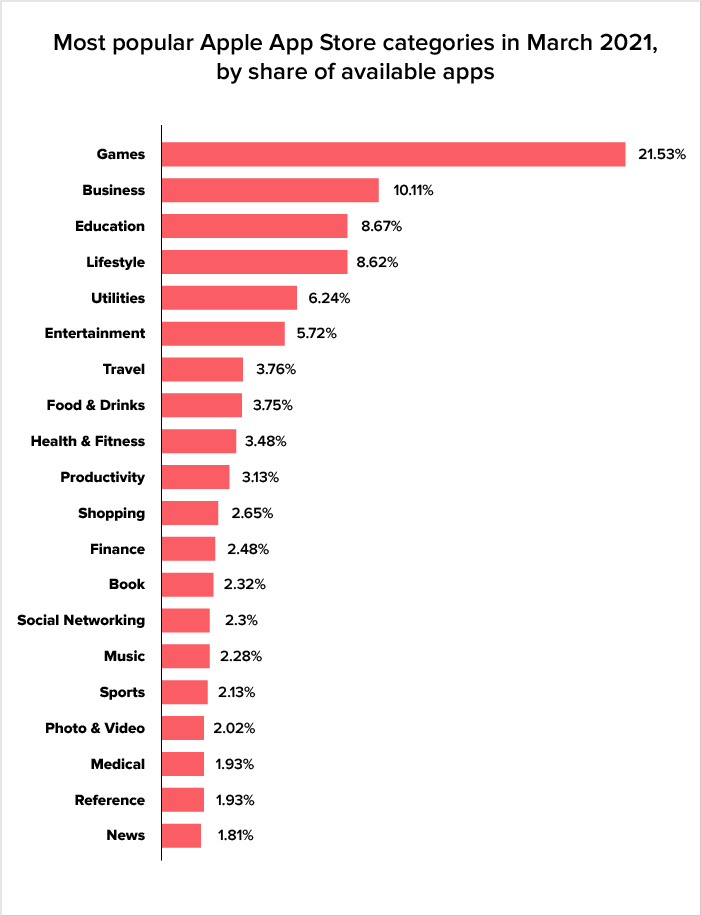
\includegraphics[width=0.95\linewidth]{00_IntroProgramacionYMoviles/TiposAplicaciones.png} 
\end{center}
\column{0.30\linewidth}
\begin{center}
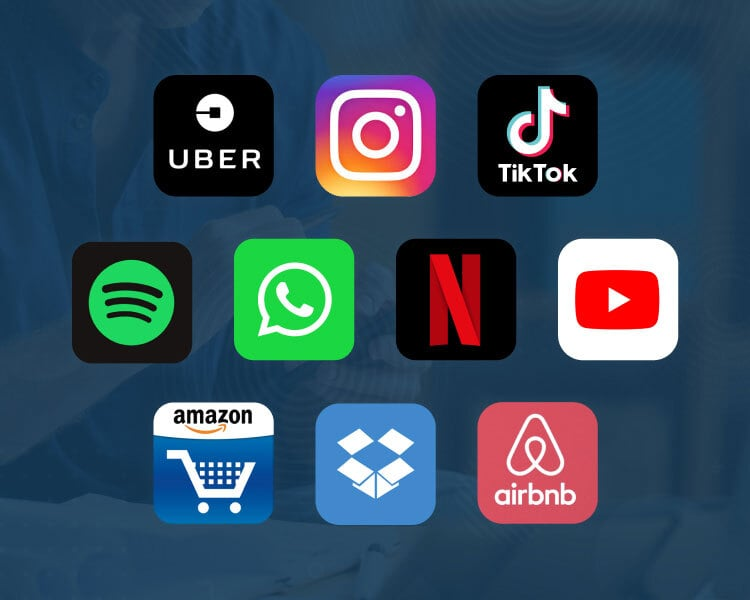
\includegraphics[width=0.95\linewidth]{00_IntroProgramacionYMoviles/most-popular-apps.jpg} 
\tiny{\url{https://www.netsolutions.com/insights/top-10-most-popular-apps-2018/}}  
\end{center}
\end{columns}
\end{frame}


\begin{frame}
\frametitle{Android Studio}  

\begin{itemize}
\item Android Studio es un entorno oficial de desarrollo integrado (IDE) para el sistema operativo Android de Google
\item La primera versi\'on se libera en el año 2013, siendo el lenguaje de programacion Java
\item En 2019, se reemplaza el lenguaje oficial de desarrollo por Kotlin, aunque Java todav\'ia es soportado
\item Es gratis, se puede descargar e instalar en cualquier computadora sin importar el sistema operativo (Windows, Linux y MacOS)
\url{https://developer.android.com}
\end{itemize}
\end{frame}

\section[HR]{Herramientas Requeridas}


\begin{frame}
\frametitle{Android Studio}  

\begin{itemize}
\item Android Studio es un entorno oficial de desarrollo integrado (IDE) para el sistema operativo Android de Google
\item La primera versi\'on se libera en el año 2013, siendo el lenguaje de programacion Java
\item En 2019, se reemplaza el lenguaje oficial de desarrollo por Kotlin, aunque Java todav\'ia es soportado
\item Es gratis, se puede descargar e instalar en cualquier computadora sin importar el sistema operativo (Windows, Linux y MacOS)
\url{https://developer.android.com}
\end{itemize}
\end{frame}





\begin{frame}
\frametitle{OpenCV para Android}  
\begin{itemize}
\item OpenCV es una librer\'ia que incluye operadores de vision por computadora en tiempo real
\item Originalmente creada por Intel en 1999
\item Es multiplataforma y open-source (Licencia Apache)
\begin{itemize}
\item Se descarga la versi\'on para Android del siguiente enlace: \url{https://opencv.org/releases/}
\item Es necesario descomprimir, ya que se va a utilizar para algunos demos que seran vistos mas adelante
\end{itemize}
\end{itemize}
\end{frame}

\begin{frame}
\frametitle{Otras herramientas software}  
Son opcionales, pero se recomienda instalarlas para una exploracion mas profunda de los conceptos que seran vistos en este curso. Todas son multiplataforma.
\begin{itemize}
\item Blender. Es un programa para modelar, renderizar y crear gr\'aficos, pudienro ser exportados a formatos OBJ y GLB. 
\item MeshViewer. Programa para visualizar archivos de gr\'aficos en formato GLB. (\url{https://github.com/RBFraphael/meshviewer/releases})
\item Scrcpy. Programa que permite duplicar en una computadora el escritorio de un tel\'efono Android conectado mediante USB
\end{itemize}
Paginas de Internet
\begin{itemize}
\item SketchFab (\url{https://sketchfab.com/}). Permite obtener modelos 3D en diferentes formatos (particularmente en GLB) -- Requiere Login con cuenta de Google, 
\item Free online OBJ to GLB converter. (\url{https://products.aspose.app/3d/conversion/obj-to-glb}) (En caso de no contar con Blender). 
\end{itemize}
\end{frame}

\begin{frame}
\frametitle{Hardware requerido}  
\begin{itemize}
\item PC con Android Studio instalado 
\item Telefono Inteligente con SO Android
\item Cable USB
\item Adaptador de Realidad Virtual (Opcional)
\item Control de Videojuego Bluetooth (Opcional)
\end{itemize}
\end{frame}


\section[PCS]{Pasos para configurar Smartphone}

%\section{Configurar smartphone en modo de Depuracion}

\begin{frame}
\frametitle{Configurar telefono inteligente en modo de desarrollador (0)}  
\begin{itemize}
\item Es necesario buscar en las opciones de configuraci\'on, en el apartado acerca del telefono ubicar el n\'umero de compilaci\'on 
\item Dar 5 taps (toques) sobre el n\'umero compilaci\'on. Debera aparecer un mensaje que diga que estas a X taps de ser un desarrollador 
\item Lo anterior habilita un nuevo men\'u en el apartado sistema dentro de opciones de configuraci\'on con t\'itulo ``opciones para desarrolladores'' 
\item Debe habilitarse tanto ``opciones para desarrolladores'' como la opci\'on ``depuraci\'on USB''
\end{itemize}

\end{frame}



\begin{frame}
\frametitle{Configurar telefono inteligente en modo de desarrollador (1)}  
\begin{columns}
\column{0.25\linewidth}
\begin{center}
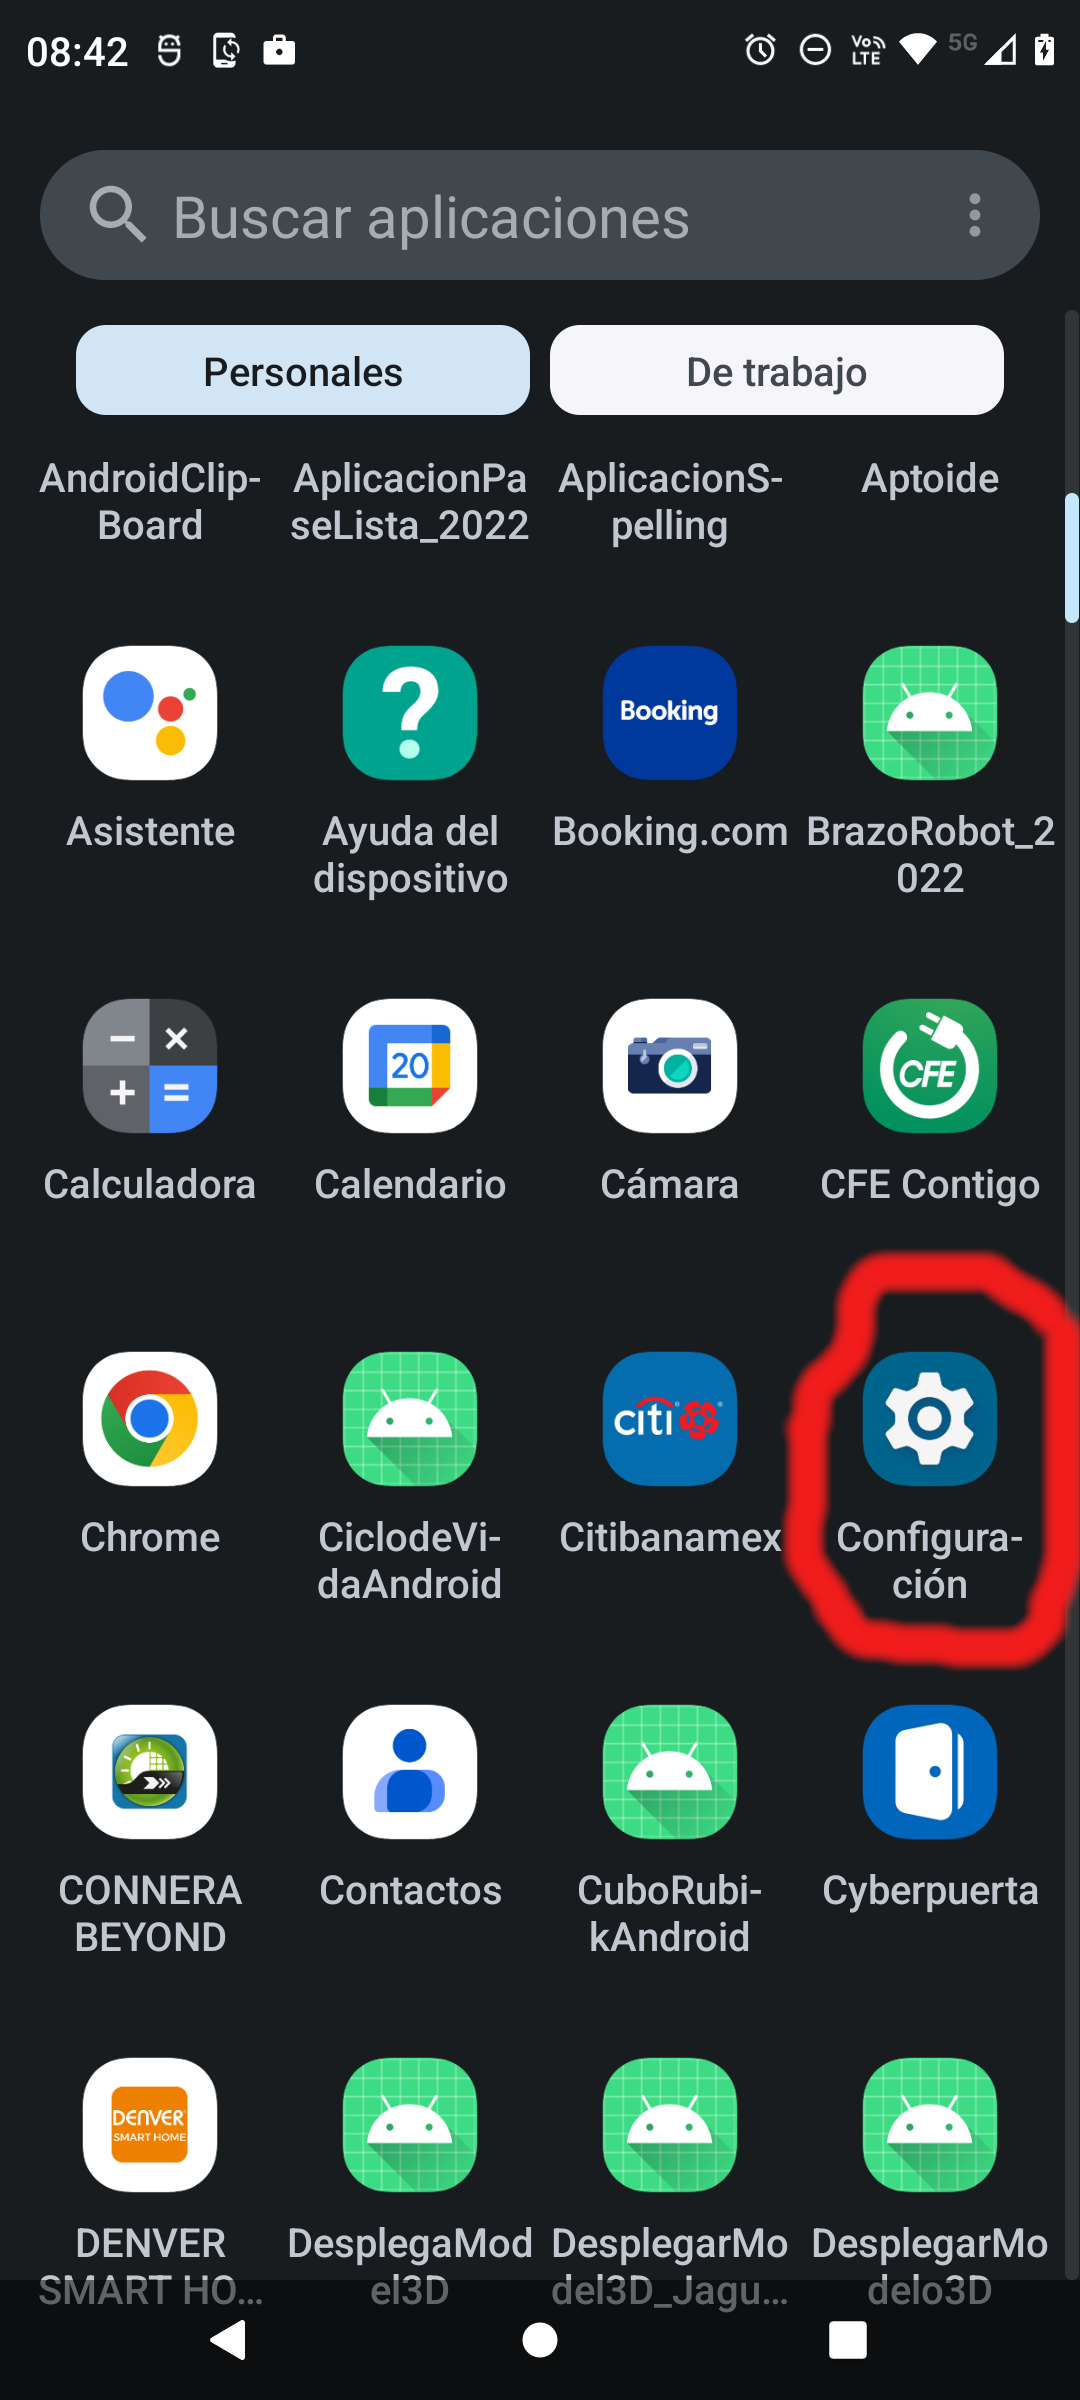
\includegraphics[width=0.95\linewidth]{01_Configurar/ModoDesarrollador1.png}    
\end{center}
\column{0.25\linewidth}
\begin{center}
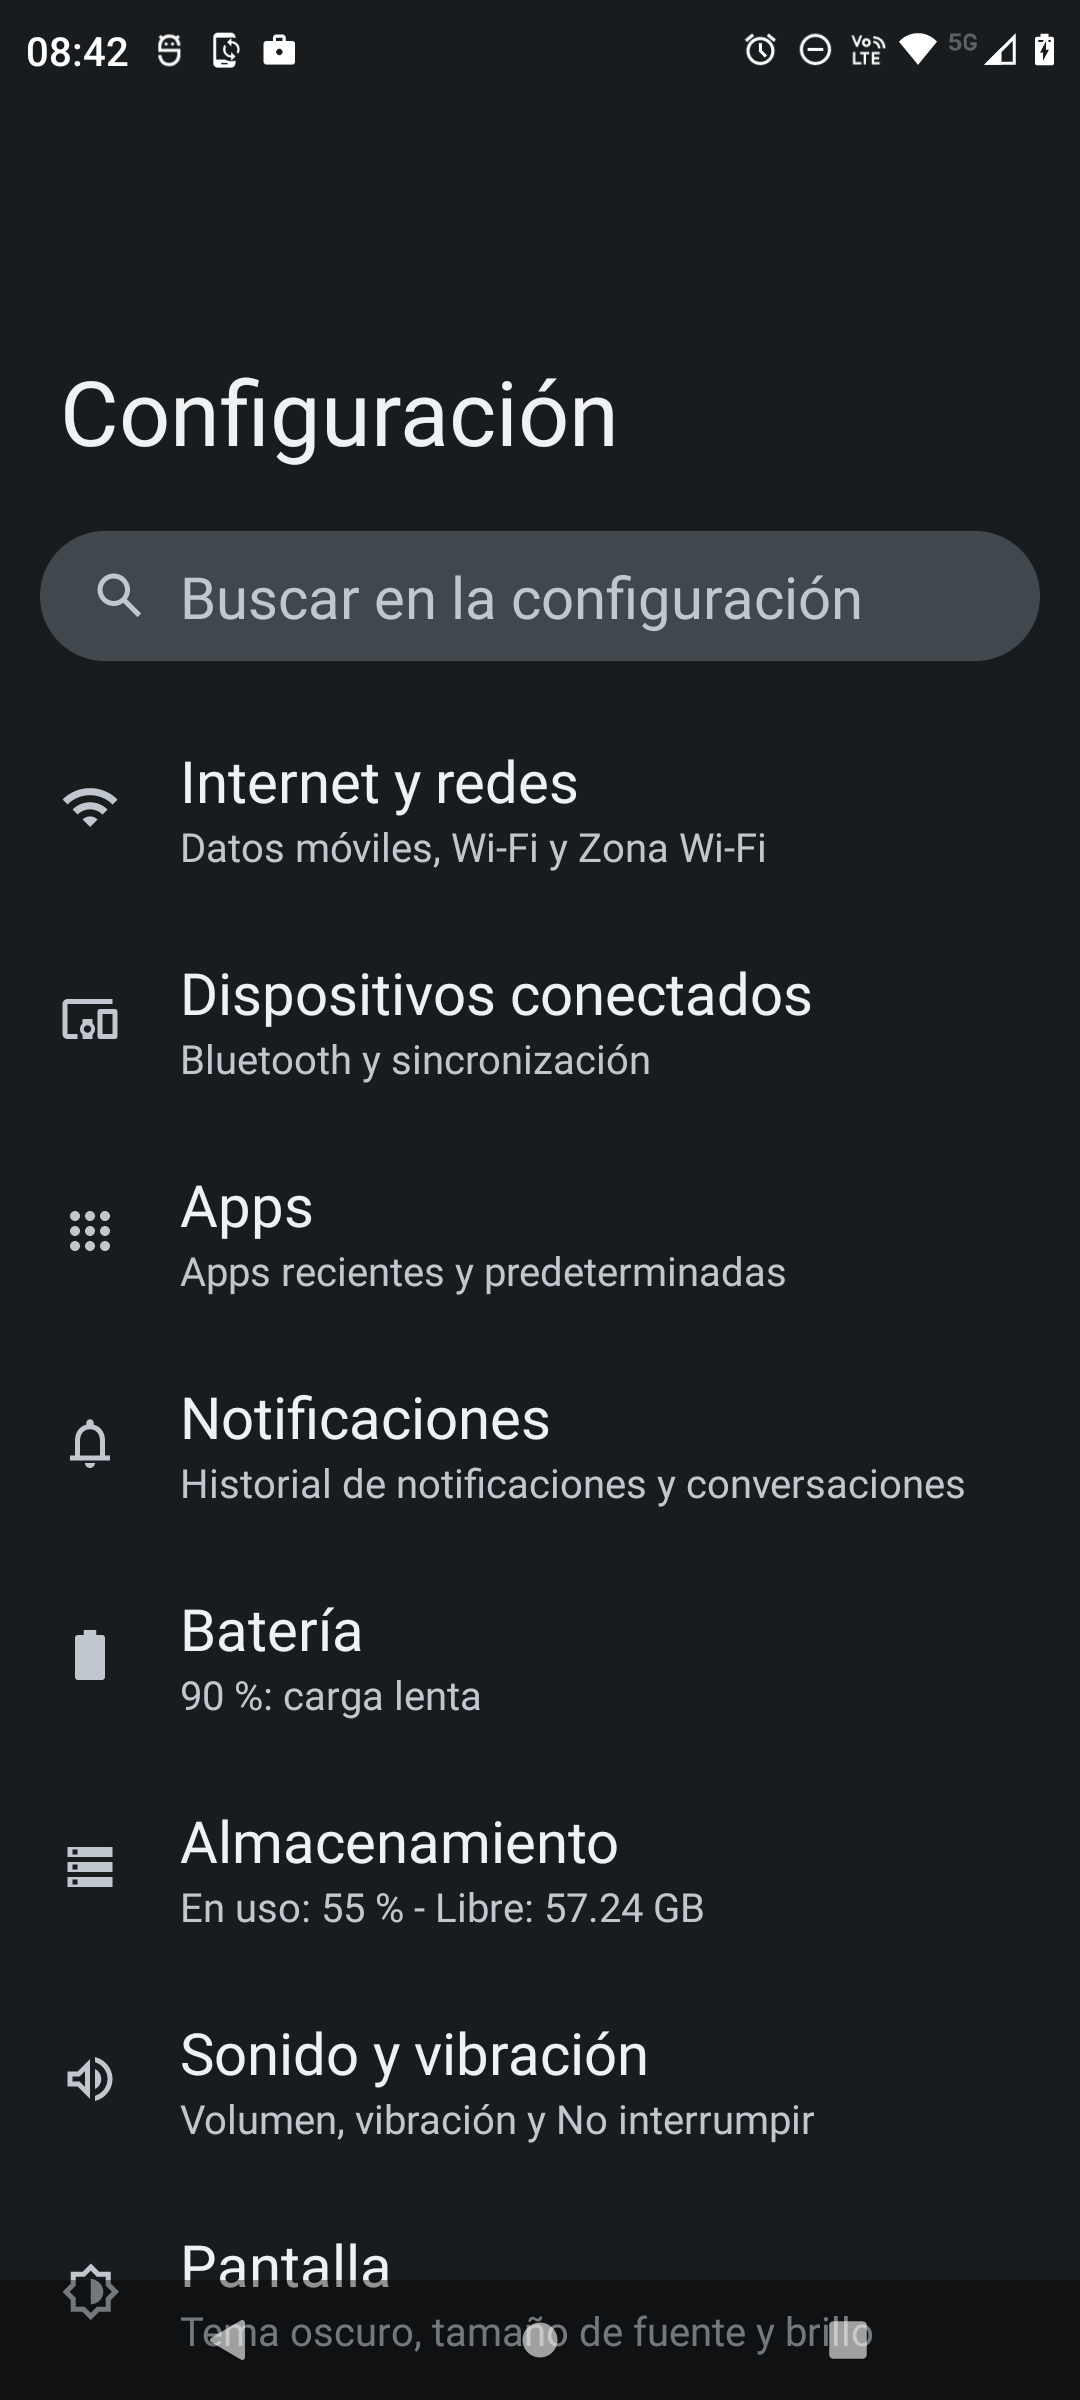
\includegraphics[width=0.95\linewidth]{01_Configurar/ModoDesarrollador2.png}    
\end{center}
\column{0.25\linewidth}
\begin{center}
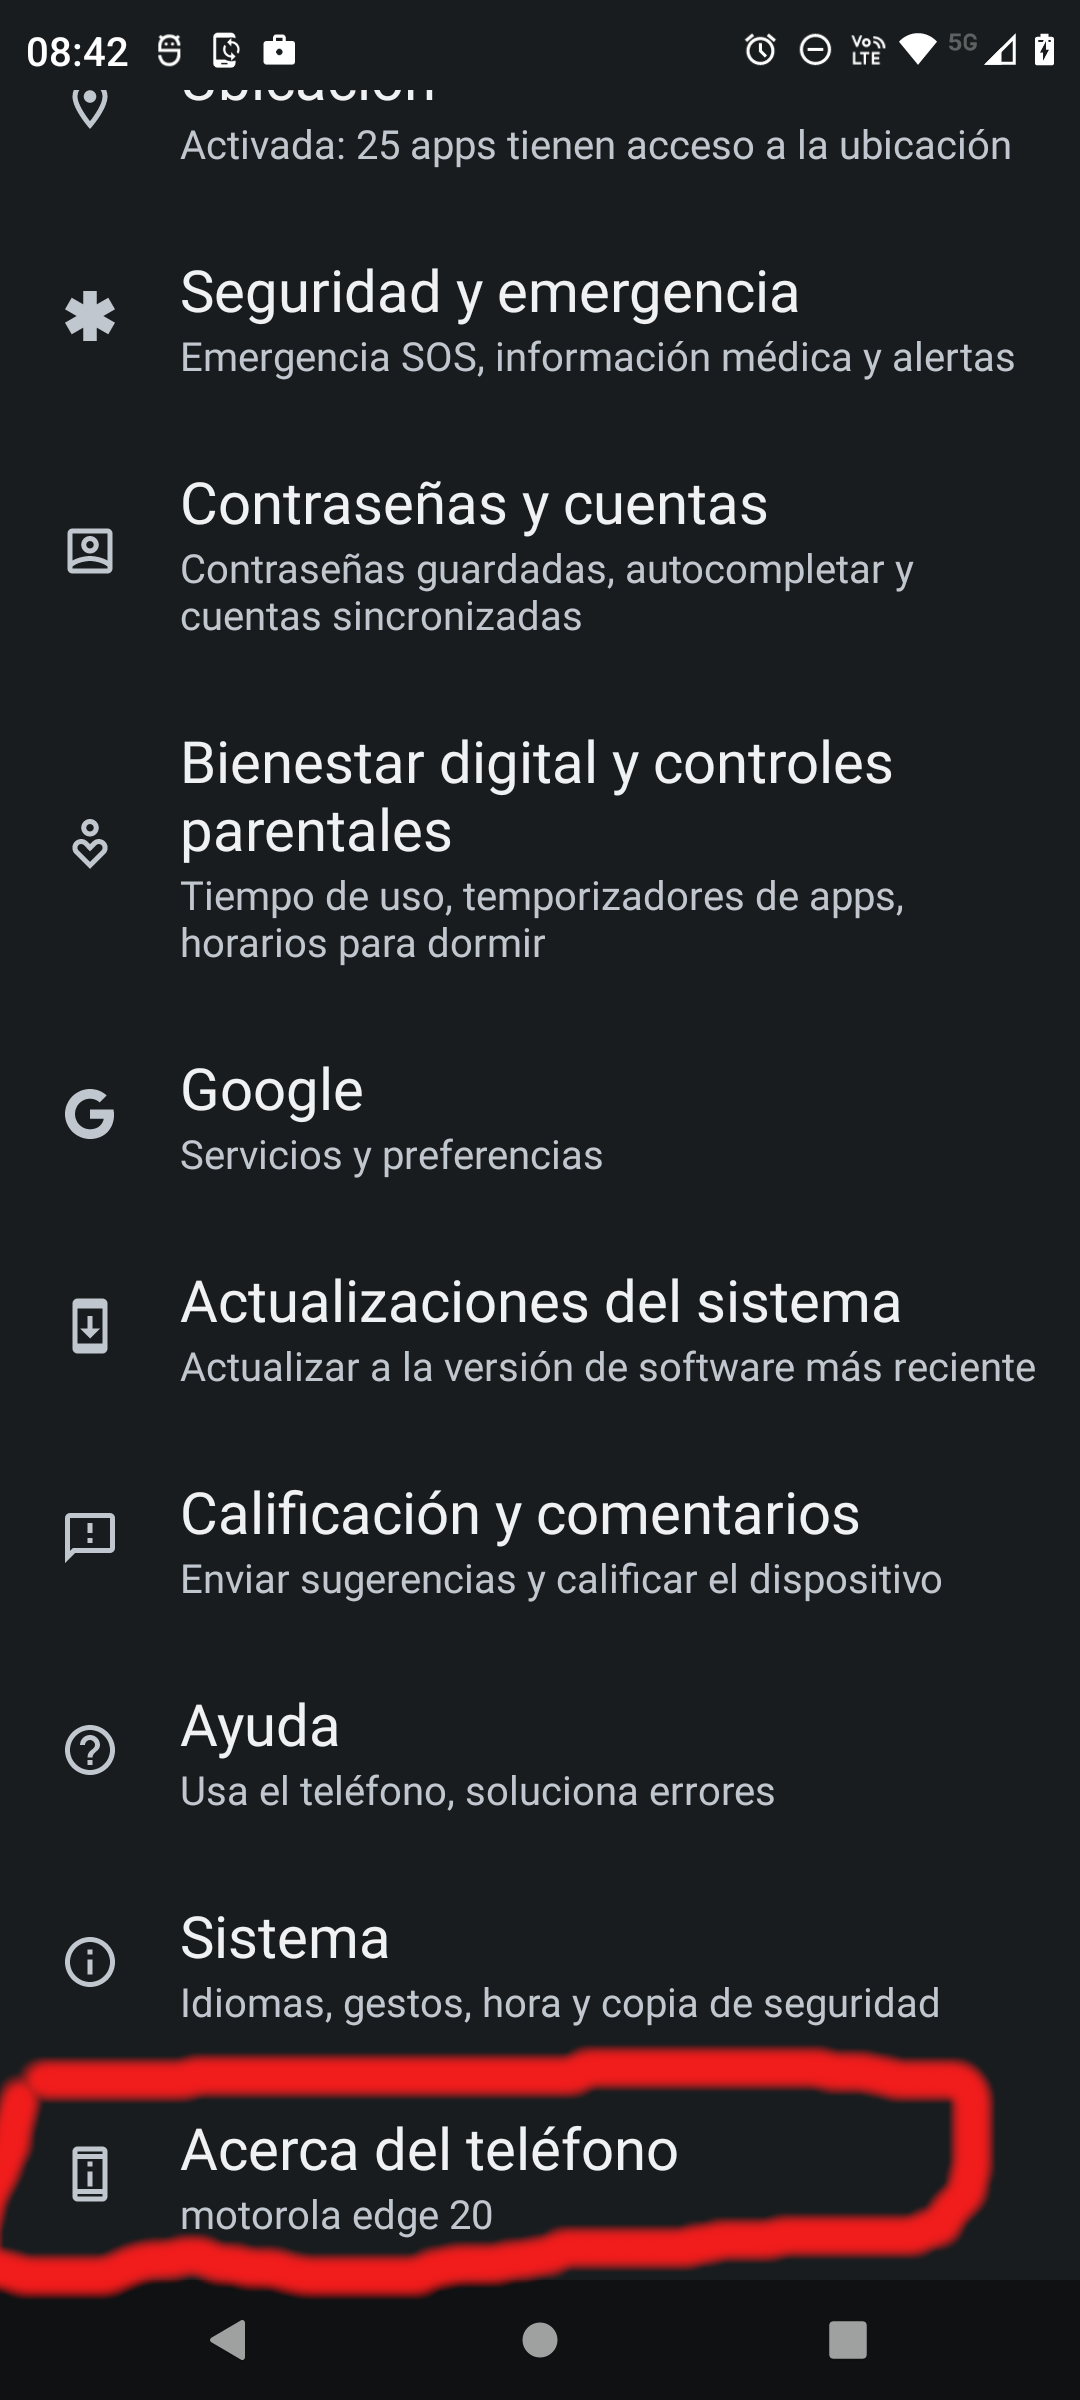
\includegraphics[width=0.95\linewidth]{01_Configurar/ModoDesarrollador3.png}    
\end{center}
\column{0.25\linewidth}
\begin{center}
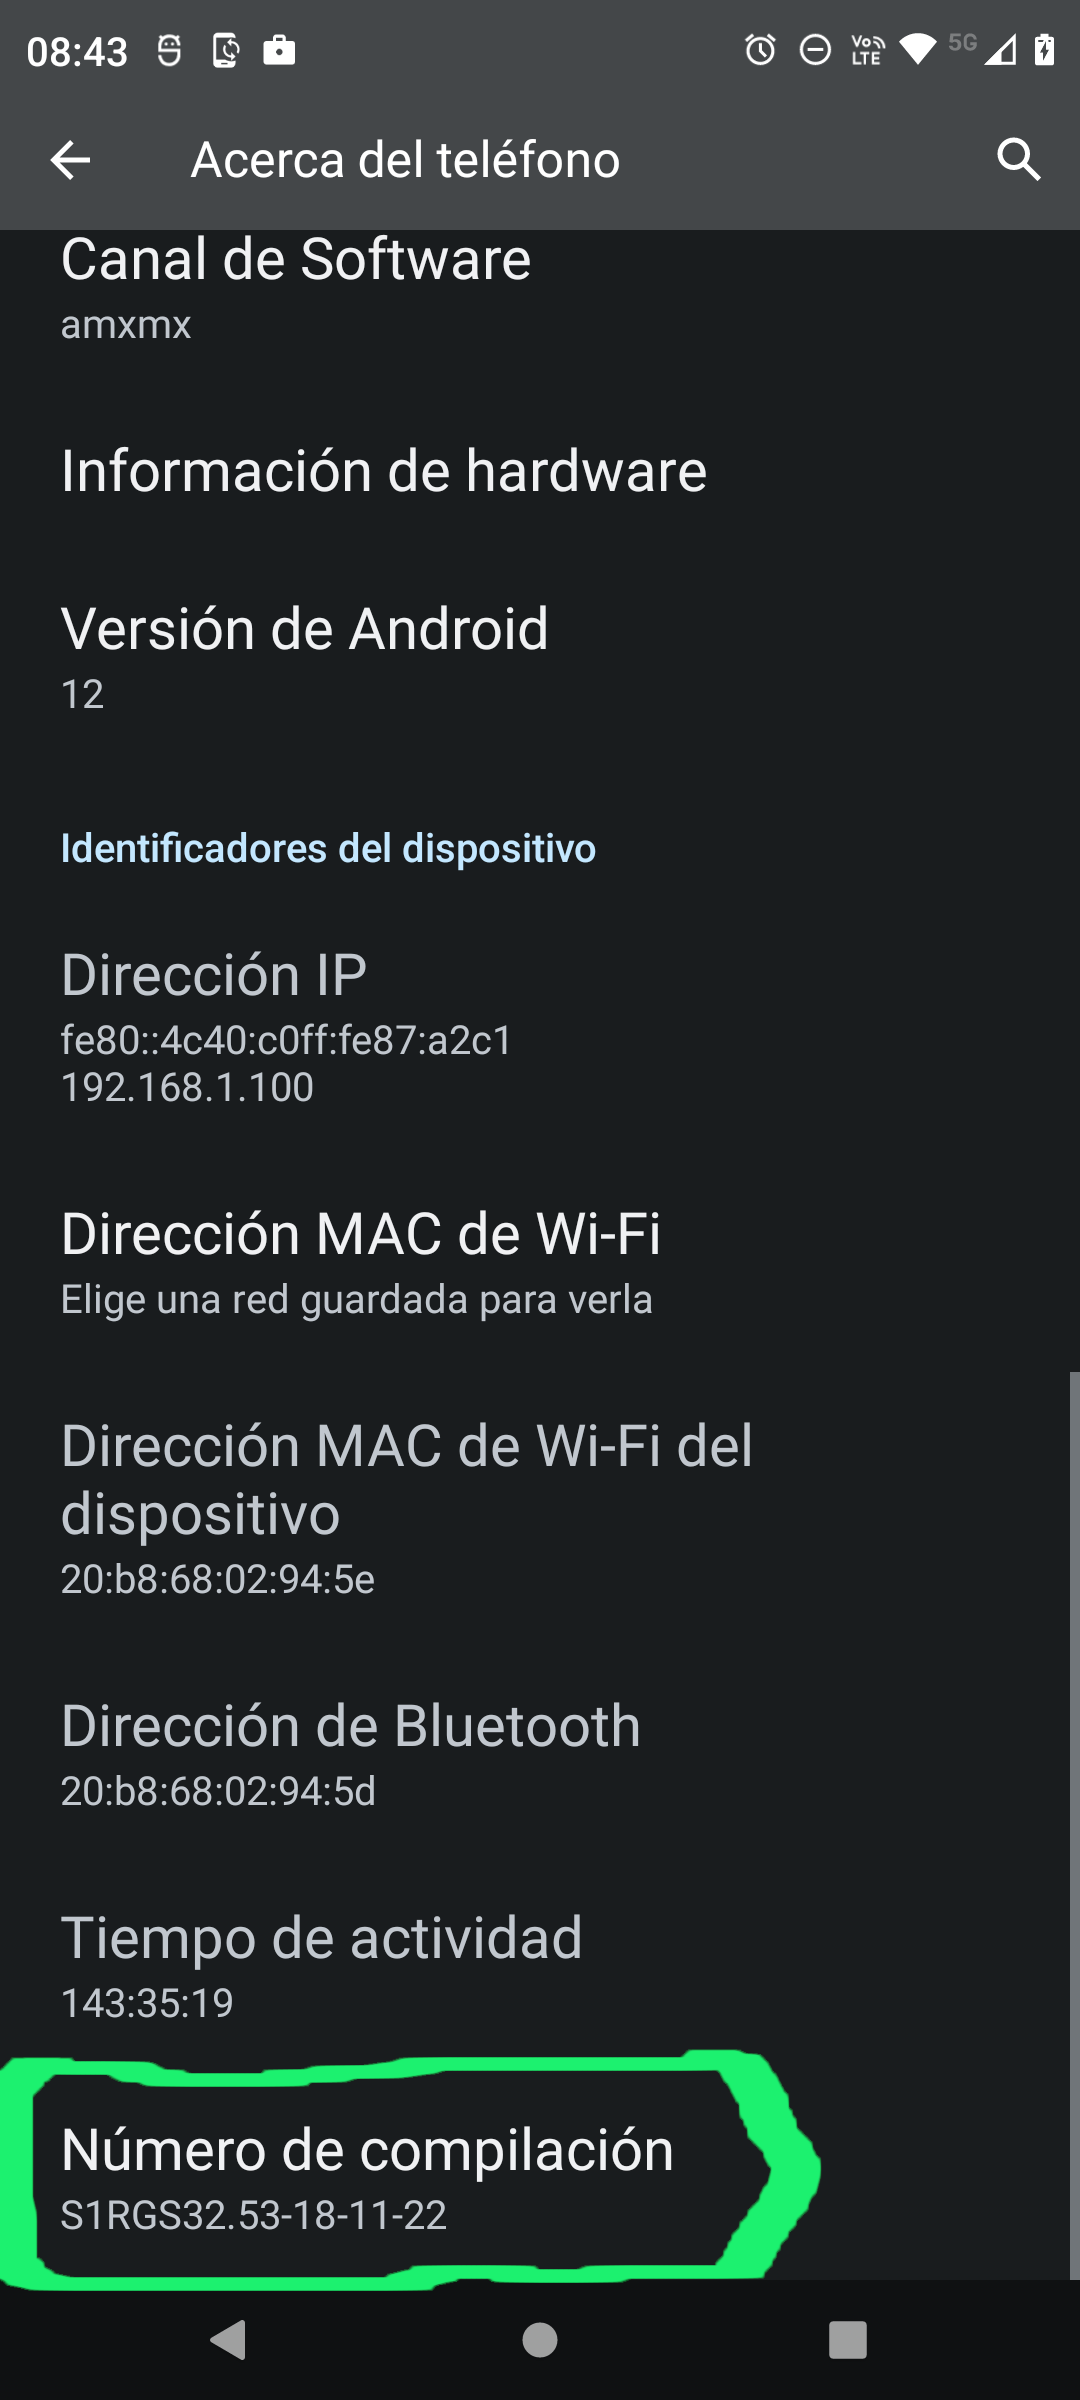
\includegraphics[width=0.95\linewidth]{01_Configurar/ModoDesarrollador4.png}    
\end{center}


\end{columns}

\end{frame}


\begin{frame}
\frametitle{Configurar telefono inteligente en modo de desarrollador (2)}  
\begin{columns}
\column{0.25\linewidth}
\begin{center}
\includegraphics[width=0.95\linewidth]{01_Configurar/ModoDesarrollador5.png}    
\end{center}
\column{0.25\linewidth}
\begin{center}
\includegraphics[width=0.95\linewidth]{01_Configurar/ModoDesarrollador6.png}    
\end{center}
\column{0.25\linewidth}
\begin{center}
\includegraphics[width=0.95\linewidth]{01_Configurar/ModoDesarrollador7.png}    
\end{center}
\column{0.25\linewidth}
\begin{center}
\includegraphics[width=0.95\linewidth]{01_Configurar/ModoDesarrollador8.png}    
\end{center}
\end{columns}
\end{frame}

\begin{frame}
\frametitle{Configurar telefono inteligente en modo de desarrollador (3)}  
\begin{columns}
\column{0.75\linewidth}

\begin{itemize}
\item Al habilitar la depuracion, aparece un mensaje de advertencia
\item Una vez que hayas terminado tus pruebas, se recomienda deshabilitar este modo de depuraci\'on
\item Para poder instalar una aplicaci\'on desarrollada con Android Studio, se debe conectar el tel\'efono inteligente a la computadora usando un cable USB
\end{itemize}

\column{0.25\linewidth}
\begin{center}
\includegraphics[width=0.95\linewidth]{01_Configurar/PermitirHabiliarOpcionesDesarrollo.jpg}    
\end{center}
\end{columns}
\end{frame}



\begin{frame}
\frametitle{Conectar smartphone a la computadora (Cable USB)}  
\begin{columns}
\column{0.25\linewidth}
\begin{itemize}
\item Al conectar el dispositivo por primera vez, aparece un mensaje de confirmaci\'on en el dispositivo
\item Configurar el telefono para que se conecte en modo de transferencia de archivos (por defecto, esta cargando)
\end{itemize}

\column{0.25\linewidth}
\begin{center}
\includegraphics[width=0.95\linewidth]{01_Configurar/HabilitarDepuracionUSB2.jpg}    
\end{center}

\column{0.25\linewidth}
\begin{center}
\includegraphics[width=0.95\linewidth]{01_Configurar/ModoConexion1.png}    
\end{center}

\column{0.25\linewidth}
\begin{center}
\includegraphics[width=0.95\linewidth]{01_Configurar/ModoConexion2.png}    
\end{center}
\end{columns}
\end{frame}







%\section{Pasos para configurar smartphone Android en modo Desarrollador}

\begin{frame}
\frametitle{Crear un primer proyecto (1)}  
\begin{columns}
\column{0.50\linewidth}
\begin{itemize}
\item Buscar el icono de la aplicacion y dar doble click
\item En caso de que requiera algunas actualizaciones, ser paciente, puede tardar.
\item Aparecera una ventana como la mostrada, seleccionar la opci\'on ``New project''
\end{itemize}
\column{0.50\linewidth}
\begin{center}
\includegraphics[width=0.95\linewidth]{01_PasosCrearProyectoAndroidStudio/AndroidStudio01.png}    
\end{center}
\end{columns}
\end{frame}

\begin{frame}
\frametitle{Crear un primer proyecto (2)}  
\begin{columns}
\column{0.50\linewidth}
\begin{itemize}
\item Existen varios tipos de dispositivos para los que pueden crearse proyectos. Por defecto nos ubica en el primer grupo (Phone and Tablet)
\item Seleccionar tipo de proyecto  ``Empty Views Activity'' y dack click en Next
\end{itemize}
\column{0.50\linewidth}
\begin{center}
\includegraphics[width=0.95\linewidth]{01_PasosCrearProyectoAndroidStudio/AndroidStudio02.png}    
\end{center}
\end{columns}
\end{frame}

\begin{frame}
\frametitle{Crear un primer proyecto (3)}  
\begin{columns}
\column{0.50\linewidth}
\begin{itemize}
\item Dejar los valores por defecto, solo se suguiere cambiar el nombre del proyecto
\item \textbf{Debe estar seleccionado como lenguaje Kotlin}. De estar seleccionado uno diferente, cambiar
\item Presionar el boton Finish
\end{itemize}
\column{0.50\linewidth}
\begin{center}
\includegraphics[width=0.95\linewidth]{01_PasosCrearProyectoAndroidStudio/AndroidStudio03.png}    
\end{center}
\end{columns}
\end{frame}

\begin{frame}
\frametitle{Crear un primer proyecto (4)}  
\begin{columns}
\column{0.50\linewidth}
\begin{itemize}
\item La primera vez que se crea un proyecto, puede requerir la descarga de archivos necesarios. Le recomiendo ser paciente
\item Ya una vez que el proyecto fue creado, aparece la ventana mostrada
\end{itemize}
\column{0.50\linewidth}
\begin{center}
\includegraphics[width=0.95\linewidth]{01_PasosCrearProyectoAndroidStudio/AndroidStudio04.png}    
\end{center}
\end{columns}
\end{frame}


\begin{frame}
\frametitle{Ejecutar proyecto en telefono inteligente} 
\begin{columns}

\column{0.75\linewidth}
\begin{itemize}
\item Una vez conectado el telefono, debe aparecer el modelo en la parte superior (lado derecho) de tu proyecto de Android Studio
\item Para instalar la aplicacion en el telefono, deber dar click en una flecha verde justo a un lado de nombre del telefono (sean pacientes, puede tardar un poco la primera vez)
\end{itemize}
\begin{center}
\includegraphics[width=0.65\linewidth]{01_PasosCrearProyectoAndroidStudio/AndroidStudio_SmartphoneReconocido.png}    
\end{center}
\column{0.25\linewidth}
\begin{center}
\includegraphics[width=0.95\linewidth]{01_PasosCrearProyectoAndroidStudio/Etapa1_fase1.png}    
\end{center}
\end{columns} 
\end{frame}





\section[PDAS]{Primer demo en Android Studio}

%\section{Modificacion de la Interfaz de usuario}


\begin{frame}
\frametitle{Carpetas del proyecto}
\begin{columns}
\column{0.75\linewidth}
Carpetas y archivos importantes
\begin{itemize}
\item \textit{Manifest} - Por el momento es de interes
\item \textit{Java} - C\'odigo fuente - Dentro hay un archivo \textit{MainActivity.kt}
\item \textit{Res} - Recursos (im\'agenes) y definici\'on de interfaces. Dentro hay una carpeta llamada \textit{layout}, con un archivo \textit{activity\_main.xml}
\end{itemize}
\column{0.25\linewidth}
\begin{center}
\includegraphics[width=0.95\linewidth]{01_Modificacion/PanelCarpetas.png}    
\end{center}
\end{columns}   
\end{frame}


%\section{Agregar Codigo a la Interfaz}
\begin{frame}[fragile]
\frametitle{Agregar codigo a la interfaz}  


\begin{columns}

\column{0.50\linewidth}
\textit{Apariencia}
\begin{block}{Archivo \textbf{activity\_main.xml}}
\begin{minted}[linenos,fontsize=\tiny]{xml}
<?xml version="1.0" encoding="utf-8"?>
<androidx.constraintlayout.widget.ConstraintLayout 
    xmlns:android="http://schemas.android.com/apk/res/android"
    xmlns:app="http://schemas.android.com/apk/res-auto"
    xmlns:tools="http://schemas.android.com/tools"
    android:layout_width="match_parent"
    android:layout_height="match_parent"
    tools:context=".MainActivity">
    <TextView
        android:layout_width="wrap_content"
        android:layout_height="wrap_content"
        android:text="Hello World!"
        app:layout_constraintBottom_toBottomOf="parent"
        app:layout_constraintEnd_toEndOf="parent"
        app:layout_constraintStart_toStartOf="parent"
        app:layout_constraintTop_toTopOf="parent" />
</androidx.constraintlayout.widget.ConstraintLayout>
\end{minted}

\end{block}

\column{0.48\linewidth}
\textit{Comportamento}
\begin{block}{Archivo \textbf{MainActivity.kt}}
\begin{minted}[linenos,fontsize=\tiny]{kotlin}
package com.example.primeraplicacionandroid
import androidx.appcompat.app.AppCompatActivity
import android.os.Bundle
class MainActivity : AppCompatActivity() {
    override fun onCreate(savedInstanceState: Bundle?) {
        super.onCreate(savedInstanceState)
        setContentView(R.layout.activity_main)
    }
}
\end{minted}
\end{block}
\end{columns}
\end{frame}

\begin{frame}
\frametitle{Interfaz de Usuario}  

\begin{columns}

\column{0.60\linewidth}
\begin{itemize}
\item Define los controles de interfaz que la aplicacion muestra
\item Estos controles pueden estar agrupados en contenedores
\item El archivo \textbf{activity\_main.xml} es la definicion del layout (la organizacion de dichos componentes)
\end{itemize}

\begin{columns}
\column{0.50\linewidth}
\begin{center}
\includegraphics[width=0.75\linewidth]{01_Modificacion/CajaContenedora.png}    
\end{center}
\column{0.50\linewidth}
\begin{center}
\includegraphics[width=0.75\linewidth]{01_Modificacion/Divisiones.jpg}    
\end{center}
\end{columns}

\column{0.40\linewidth}

\begin{center}
\includegraphics[width=0.95\linewidth]{01_Modificacion/ElementosInterfaz.png}    
\end{center}

\end{columns}

\end{frame}


\begin{frame}[fragile]
\frametitle{Primer modificaci\'on}

\begin{columns}
\column{0.48\linewidth}
\begin{block}{Archivo Original \textbf{activity\_main.xml}}
\begin{minted}[highlightlines={2,10,13-17},linenos,fontsize=\tiny]{xml}
<?xml version="1.0" encoding="utf-8"?>
<androidx.constraintlayout.widget.ConstraintLayout 
    xmlns:android="http://schemas.android.com/apk/res/android"
    xmlns:app="http://schemas.android.com/apk/res-auto"
    xmlns:tools="http://schemas.android.com/tools"
    android:layout_width="match_parent"
    android:layout_height="match_parent"
    tools:context=".MainActivity">
    <TextView
        android:layout_width="wrap_content"
        android:layout_height="wrap_content"
        android:text="Hello World!"
        app:layout_constraintBottom_toBottomOf="parent"
        app:layout_constraintEnd_toEndOf="parent"
        app:layout_constraintStart_toStartOf="parent"
        app:layout_constraintTop_toTopOf="parent" />
</androidx.constraintlayout.widget.ConstraintLayout>
\end{minted}
\end{block}
\column{0.48\linewidth}
\begin{block}{Archivo Modificado \textbf{activity\_main.xml}}
\begin{minted}[highlightlines={2,15,8,11,12},linenos,fontsize=\tiny]{xml}
<?xml version="1.0" encoding="utf-8"?>
<LinearLayout 
    xmlns:android="http://schemas.android.com/apk/res/android"
    xmlns:app="http://schemas.android.com/apk/res-auto"
    xmlns:tools="http://schemas.android.com/tools"
    android:layout_width="match_parent"
    android:layout_height="match_parent"
    android:orientation="vertical"
    tools:context=".MainActivity">
    <TextView
        android:background="#00ffff"
        android:layout_width="match_content"
        android:layout_height="wrap_content"
        android:text="Hello World!" />
</LinearLayout>


\end{minted}
\end{block}
\end{columns}
\end{frame}




\begin{frame}[fragile]
\frametitle{Primer modificaci\'on}

\begin{columns}
\column{0.80\linewidth}
\begin{enumerate}
\item Reemplazar \textit{androidx.constraintlayout.widget.ConstraintLayout} por \textit{LinearLayout}
\begin{itemize}
\item Tipo de contenedor donde los componentes se agregan secuencialmente
\end{itemize}
\item Agregar propiedad \textit{android:orientation=``vertical''} al \textit{LinearLayout} principal
\begin{itemize}
\item Los componentes seran ordenados verticalmente
\end{itemize}
\item Cambiar la propiedad \textit{android:layout\_width="wrap\_content"} por \textit{android:layout\_width=``match\_parent''}
\begin{itemize}
\item El ancho de TextView abarcar toda la pantalla
\end{itemize}
\item Agregar la propiedad \textit{android:background=``\#00ffff'' al textview} - 
\begin{itemize}
\item La cadena ``\#00ffff'' define el color azul. Se pueden probar con otros buscando en Internet un generador de colores hexadecimal y cambiando por otros de tu preferencia
\end{itemize}
\end{enumerate}
\column{0.20\linewidth}

\begin{center}
\includegraphics[width=0.95\linewidth]{01_Modificacion/App_Version2.png}    
\end{center}
\end{columns}
\end{frame}


\section[PRVA]{Prototipos de Aplicaciones Graficas y de VC}


\renewcommand{\EntradaBibtex}{Ajedrez3D_2017}
%\setcounter{footnote}{0}


\begin{frame}{\citetitle{\EntradaBibtex} \footnotemark[1] (1)}
%\begin{block}{Multiplayer Chess \footnotemark} 
\begin{columns}
\begin{column}{0.4\textwidth}
		\begin{itemize}
		\item Cada pieza fue modelada en Blender y exportada a la aplicación de Android
		\item Aplicación multidispositivo, que permite llevar una partida de ajedrez.
		\item El control del juego queda del lado del servidor. 
		\end{itemize}

\end{column}
\begin{column}{0.3\textwidth}
%   some text here some text here some text here some text here some text here
     \begin{center}
     %%%%% this is a minipage, so \textwidth is already adjusted to the size of the column
     \includegraphics[width=0.7\textwidth]{Figs/Ajedrez_01}
     \end{center}

\end{column}
\begin{column}{0.3\textwidth}  
    \begin{center}
     %%%%% this is a minipage, so \textwidth is already adjusted to the size of the column
     \includegraphics[width=0.7\textwidth]{Figs/Ajedrez_02}
     \end{center}
\end{column}
\end{columns}
%\footfullcite*{\EntradaBibtex}
\footnotetext[1]{\fullcite{\EntradaBibtex}}
\end{frame}



\renewcommand{\EntradaBibtex}{CruzdeMalta_2017}

\begin{frame}{\citetitle{\EntradaBibtex} \footnotemark[1] (1)}
%\begin{block}{Simulación del Mecanismo de la Cruz de Malta\footnotemark} 
	\begin{itemize}
	\item Se modelaron los componentes individuales 3D (cilindros, tetaedros, etc)
	\item Se incorporó texturas, iluminación y sombras
	\item Es posible ver el modelo desde múltiples perspectivas
	\end{itemize}
\begin{columns}
	\begin{column}{0.48\textwidth}
    \begin{center}
     \includegraphics[width=0.7\textwidth]{Figs/CruzMalta_01}
     \end{center}
\end{column}
\begin{column}{0.48\textwidth}  
    \begin{center}
     \includegraphics[width=0.7\textwidth]{Figs/CruzMalta_02}
     \end{center}
\end{column}
\end{columns}
%\end{block} 
\footnotetext[1]{\fullcite{\EntradaBibtex}}
%\footnotetext{Héctor Hugo Sandoval Marcelo. \textbf{Movimiento de la Cruz de Malta con Iluminación y Texturas con Java y OpenGL ES 2.0 en Android.}. Universidad Politécnica de Victoria,  Informe técnico proyecto de asignatura ``Graficación por Computadora Avanzada'', 2017. Sin Publicar.}
%\\setcounter{footnote}{0}
\end{frame}




\renewcommand{\EntradaBibtex}{Reporte2017_Tetris3D}

\begin{frame}{\citetitle{\EntradaBibtex} \footnotemark[1] (1)}
\begin{block}{Motivación} 
Este proyecto esta inspirado en un tetris 3D para PC \url{http://users.csc.calpoly.edu/~zwood/teaching/csc471/finalproj24/gzipkin/}
\begin{itemize}
\item Varias piezas caen sobre una rejilla y el objetivo es borar las lineas.
\item Las piezas se mueven en un entorno tridimensional (ejes X, Y y Z)
\item Las fronteras de la red estan definidas mediante una malla alámbrica
\item La cámara tambien se puede mover en base a eventos de toque sobre la pantalla del dispositivo
\end{itemize}
\end{block} 
\footnotetext[1]{\fullcite{\EntradaBibtex}}
\end{frame}


\begin{frame}{Aplicación Tetris 3D (2)}
%\begin{block}{Pantallas Principales} 
\begin{center}
	\begin{tabular}{cccc}
		\includegraphics[width=0.20\linewidth]{2017_Tetris3D/figs/Tetris0.png} &
		\includegraphics[width=0.20\linewidth]{2017_Tetris3D/figs/Tetris1.png} & 		 		
		\includegraphics[width=0.20\linewidth]{2017_Tetris3D/figs/Tetris2.png} & 		
		\includegraphics[width=0.20\linewidth]{2017_Tetris3D/figs/Tetris3.png} \\
	\end{tabular}
\end{center}
\end{frame}








\begin{frame}{\citetitle{MarcoNuno_Revista_2020_10_00} \footnotemark (1)}

\begin{columns}
\begin{column}{0.5\textwidth}
	\begin{itemize}
\item Es necesario herramientas para educar a pacientes con Diabetes para manejar su enfermedad.
\item Se propone una aplicación móvil que permita generar una simulación del comportamiento de la glucosa en un organismo con Diabetes a partir de modelos:
	\begin{itemize}
		\item Dosificación de insulina
		\item Ejercicio
		\item Ingesta de alimentos
	\end{itemize}
	\end{itemize}
\end{column}
\begin{column}{0.5\textwidth}
\begin{center}
     %%%%% this is a minipage, so \textwidth is already adjusted to the size of the column
     \includegraphics[width=0.99\textwidth]{Figs/Diabetes1}
     \end{center}
\end{column}
\end{columns}
\footnotetext[1]{\fullcite{MarcoNuno_Revista_2020_10_00}}
\setcounter{footnote}{0}
\end{frame}

\begin{frame}{\citetitle{MarcoNuno_Revista_2020_10_00} (2)}
\begin{columns}
\begin{column}{0.65\textwidth}
Pantallas de la aplicación:
	\begin{enumerate}
\item Pantalla inicial
\item Configuración de ingesta de alimentos
\item Configuración de dosificación de insulina
\item Configuración de configuración de rutina de ejercicio
\item Inicio de simulación
	\end{enumerate}
\end{column}
\begin{column}{0.40\textwidth}
\begin{center}
     %%%%% this is a minipage, so \textwidth is already adjusted to the size of the column
     \includegraphics[width=0.99\textwidth]{Figs/Diabetes3}
     \includegraphics[width=0.66\textwidth]{Figs/Diabetes4}
     \end{center}
\end{column}
\end{columns}
\end{frame}

\begin{frame}{\citetitle{MarcoNuno_Revista_2020_10_00} (3) } 
\begin{columns}
\begin{column}{0.65\textwidth}
La aplicación genera una gráfica de comportamiento de la glucosa a lo largo del tiempo de simulación. Se muestran las gráficas para cuatro casos:
	\begin{itemize}
\item Pacientes controlados en cuanto a los niveles de glucosa (a y b)
\item Pacientes fuera de control debido a la falta de ejercicio y al exceso de carbohidratos (c y d)
	\end{itemize}
\end{column}
\begin{column}{0.35\textwidth}
\begin{center}
     %%%%% this is a minipage, so \textwidth is already adjusted to the size of the column
     \includegraphics[width=0.99\textwidth]{Figs/Diabetes5}
     \end{center}
\end{column}
\end{columns}
\end{frame}




\begin{frame}{Detección de movimientos en un tablero de ajedrez \footnotemark}
%\begin{block}{Detección de movimientos en un tablero de ajedrez \footnotemark} 
\begin{columns}
\begin{column}{0.38\textwidth}
Aplicación de escritorio:
	\begin{itemize}
\item Entorno semicontrolado con una cámara y una Laptop con OpenCV
\item Detecta las esquinas del tablero de ajedrez
\item Transformada de Hough
\item Detectar si hay casilla o no dentro de la región de interés
	\end{itemize}
\end{column}
\begin{column}{0.28\textwidth}
\begin{center}
     %%%%% this is a minipage, so \textwidth is already adjusted to the size of the column
     \includegraphics[width=0.75\textwidth]{Figs/AjedrezFroylan1}\\
%     \includegraphics[width=0.35\textwidth]{Figs/AjedrezFroylan2}
     \end{center}
\end{column}
\begin{column}{0.28\textwidth}
\begin{center}
     %%%%% this is a minipage, so \textwidth is already adjusted to the size of the column
 %    \includegraphics[width=0.35\textwidth]{Figs/AjedrezFroylan1}\\
     \includegraphics[width=0.75\textwidth]{Figs/AjedrezFroylan2}
     \end{center}
\end{column}

\end{columns}
%\end{block} 
\footnotetext{\fullcite{Froylan_VC_2021}}
%\footnotetext{Froylan Melquiades Wbario Martinez, \textbf{Seguidor de movimientos de Ajedrez}. Universidad Politécnica de Victoria, Informe técnico proyecto de asignatura “Visión por Computadora”, 2021.  En evaluación.}
%\\setcounter{footnote}{0}
\end{frame}

\begin{frame}{Detección de movimientos en un tablero de ajedrez (2)}
%\begin{block}{Detección de movimientos en un tablero de ajedrez (2)} 
\begin{columns}
\begin{column}{0.38\textwidth}
Aplicación de escritorio:
	\begin{itemize}
\item Una vez detectadas las regiones, se emplea un cronometro para determinar la diferencia entre dos instantaneas consecutivas
\item Problemas actuales: Iluminación, sombras, oclusiones
	\end{itemize}
\end{column}
\begin{column}{0.28\textwidth}
\begin{center}
     %%%%% this is a minipage, so \textwidth is already adjusted to the size of the column
     \includegraphics[width=0.79\textwidth]{Figs/AjedrezFroylan3}\\
%     \includegraphics[width=0.49\textwidth]{Figs/AjedrezFroylan4}
     \end{center}
\end{column}
\begin{column}{0.28\textwidth}
\begin{center}
     %%%%% this is a minipage, so \textwidth is already adjusted to the size of the column
%     \includegraphics[width=0.49\textwidth]{Figs/AjedrezFroylan3}\\
     \includegraphics[width=0.79\textwidth]{Figs/AjedrezFroylan4}
     \end{center}
\end{column}

\end{columns}
%\end{block} 
\end{frame}






\begin{frame}{\citetitle{Avatar3d_Echartea_2021} \footnotemark (1)}
%\begin{block}{Aplicación Movil para Concientizar a Niños Acerca del Cuidado del Peso (1)} 
	\begin{itemize}
\item Se requieren herramientas que apoyen en la concientización de problemas médicos graves (Obesidad)
\item Se integra una aplicación móvil que muestre un avatar tridimensional cuyo peso, estatura y edad sea configurable con por usuario
\item Es posible configurar el numero de comidas y el tipo de ejercicio de la simulación
\item Al finalizar la simulación, la aplicación mostrará el antes o despues basado en en los IMCs y los parametros del avatar. 
\item Herramientas utilizadas
	\begin{itemize}
		\item Unity
		\item MakeHuman 
	\end{itemize}
	\end{itemize}
%\end{block} 
\footnotetext[1]{\fullcite{Avatar3d_Echartea_2021}}
\setcounter{footnote}{0}
\end{frame}

\begin{frame}{\citetitle{Avatar3d_Echartea_2021} (2)}
%\begin{block}{Simulación de modelo de diabetes en un dispositivo móvil (2)} 
\begin{center}
     \begin{tabular}{ccc}
         \includegraphics[width=0.25\textwidth]{Figs/Echartea1}&
         \includegraphics[width=0.25\textwidth]{Figs/Echartea2}&
         \includegraphics[width=0.25\textwidth]{Figs/Echartea3}\\
          \end{tabular}
\end{center}
%\end{block} 
\end{frame}

%\begin{frame}{Proyectos de Investigación}
\begin{frame}{\citetitle{Avatar3d_Echartea_2021} (3)}
%\begin{block}{Simulación de modelo de diabetes en un dispositivo móvil (2)} 
\begin{center}
     \begin{tabular}{cc}
         \includegraphics[width=0.25\textwidth]{Figs/Echartea4}&
         \includegraphics[width=0.25\textwidth]{Figs/Echartea5}
          \end{tabular}
\end{center}
%\end{block} 
\end{frame}



\begin{frame}{\citetitle{Escanner3D_Aleman2022}$^*$  (1)}
\begin{columns}
\begin{column}{0.6\textwidth}
	\begin{itemize}
		\item Muchas de las tareas que tradicionalmente se hacían en una PC ahora han migrado hacia el teléfono inteligente
        \item La digitalización de objetos 3D ha tenido un auge en tiempos recientes
		\item El escaner se obtiene datos de un sensor ultrasónico montado en un motor (escaneo vertical)
		\item Una plataforma giratoria rota el objeto para obtener los datos desde todos los ángulos
	\end{itemize}
\end{column}
\begin{column}{0.4\textwidth}  
\begin{center}
     \begin{tabular}{c}
\includegraphics[width=0.68\textwidth]{2022_Scanner3D/figs/Esc1}\\
\includegraphics[width=0.68\textwidth]{2022_Scanner3D/figs/Esc2}\\         
      \end{tabular}
\end{center}
\end{column} 
\end{columns} 
\footfullcite*{Escanner3D_Aleman2022}
\end{frame}


\begin{frame}{\citetitle{Escanner3D_Aleman2022} (2)}
	\begin{itemize}
        \item La aplicación visualiza el modelo adquirido y lo almacena en un formato estándar
        \item Se propone una App para un escaner 3D ``casero'' mediante comunicación Bluetooth
	\end{itemize}
\begin{center}
 \begin{tabular}{cccc}
    \includegraphics[width=0.14\textwidth]{2022_Scanner3D/figs/Ap1}
    \includegraphics[width=0.14\textwidth]{2022_Scanner3D/figs/Ap2}
    \includegraphics[width=0.14\textwidth]{2022_Scanner3D/figs/Ap3}
    \includegraphics[width=0.16\textwidth]{2022_Scanner3D/figs/Ap4}
  \end{tabular}
\end{center}

\end{frame}








\renewcommand{\EntradaBibtex}{BrazoRobot_Morin2019}
\begin{frame}{\citetitle{\EntradaBibtex} \footnotemark[1] (1)}
%\begin{block}{Brazo Robótico \footnotemark} 
\begin{columns}
	\begin{column}{0.55\textwidth}
		\begin{itemize}
			\item Se retoma un diseño previamente realizado para WebGL. 
			\item Los componentes del robot son movidos mediante motores, y puede ser visto desde difentes perspectivas.		
		\end{itemize}
	\end{column}
	\begin{column}{0.22\textwidth}
		 \begin{center}
		     \includegraphics[width=0.98\textwidth]{Figs/brazoRobotico1}
		 \end{center}
	\end{column}
	\begin{column}{0.22\textwidth}  
		\begin{center}
		 \includegraphics[width=0.98\textwidth]{Figs/brazoRobotico2}
		 \end{center}
	\end{column}
\end{columns}
%\end{block} 
\footnotetext[1]{\fullcite{\EntradaBibtex}}
\end{frame}

\renewcommand{\EntradaBibtex}{BrazoRobot_Uriegas2022}

\begin{frame}{\citetitle{\EntradaBibtex} \footnotemark[1] (1)}
\begin{columns}
\begin{column}{0.25\textwidth}  
\includegraphics[width=0.82\textwidth]{2019_BrazoRobot3D/figs/BrazoRobot1}
\end{column}
\begin{column}{0.25\textwidth}  
\includegraphics[width=0.82\textwidth]{2019_BrazoRobot3D/figs/BrazoRobot2}
\end{column}
\begin{column}{0.25\textwidth}  
\includegraphics[width=0.82\textwidth]{2019_BrazoRobot3D/figs/BrazoRobot3}
\end{column}
\begin{column}{0.25\textwidth}  
\includegraphics[width=0.82\textwidth]{2019_BrazoRobot3D/figs/BrazoRobot4}
\end{column}

\end{columns}
\footnotetext[1]{\fullcite{\EntradaBibtex}}
\end{frame}



\begin{frame}{\citetitle{MarcoNuno_Revista_2022_10_00}$^*$ (1)}
\begin{columns}
\begin{column}{0.99\textwidth}
	\begin{itemize}  %del cuerpo académico Acuicultura Sustentable (UTMTB-CA-1)
        \item Una aplicación eficaz para uso de transporte publico debe mostrar información acerca de las opciones de movilidad el usuario tiene en una localidad específica.
        \item En algunas localidades, esta información no esta disponible en las aplicaciones de mapas, lo que complica la movilidad del usuario.
		\item Se implementó una App específicamente para Ciudad Victoria, Tamps
	\end{itemize}
\end{column}
%\begin{column}{0.25\textwidth}  
%\includegraphics[width=0.98\textwidth]{2022_HidroponicosDavid/figs/dft}
%\end{column}
%\begin{column}{0.25\textwidth}
%\includegraphics[width=0.98\textwidth]{2022_HidroponicosDavid/figs/iot}
%\end{column}
\end{columns} 
\footfullcite*{MarcoNuno_Revista_2022_10_00}
\end{frame}


\begin{frame}{\citetitle{MarcoNuno_Revista_2022_10_00} (2)}
\begin{columns}
\begin{column}{0.25\textwidth}  
\includegraphics[width=0.82\textwidth]{2022_MapaVickyRanch/figs/F3}
\end{column}
\begin{column}{0.25\textwidth}  
\includegraphics[width=0.82\textwidth]{2022_MapaVickyRanch/figs/F4}
\end{column}
\begin{column}{0.25\textwidth}  
\includegraphics[width=0.82\textwidth]{2022_MapaVickyRanch/figs/F9}
\end{column}
\begin{column}{0.25\textwidth}  
\includegraphics[width=0.82\textwidth]{2022_MapaVickyRanch/figs/F13}
\end{column}

\end{columns} 
\end{frame}



\section[PRVA]{Prototipos de Realidad Virtual y Aumentada}

\begin{frame}{\citetitle{MarcoNuno_CongArbEsp_2013_11_01} \footnotemark (1)}
%\begin{block}{Prototipo de un entorno virtual para un robot de servicio\footnotemark } 
\begin{columns}
\begin{column}{0.52\textwidth}
    \begin{center}

\begin{itemize}
\item Prototipo SerBot I
\item Modelo 3D del Robot
\item Modelo 3D del entorno
\item Plataforma: PC de escritorio
\end{itemize}
     \end{center}

\end{column}
\begin{column}{0.48\textwidth}  
    \begin{center}
\begin{itemize}
\end{itemize}
     \includegraphics[width=0.9\textwidth]{Figs/SerbotI_A}\\
     \end{center}
\end{column}
\end{columns}


%\end{block} 
\footnotetext{\fullcite{MarcoNuno_CongArbEsp_2013_11_01}}
%\\setcounter{footnote}{0}
\end{frame}



\begin{frame}{\citetitle{MarcoNuno_CongArbEsp_2013_11_01} (2)}
%\begin{block}{Prototipo de un entorno virtual para un robot de servicio (2)} 
\begin{columns}
\begin{column}{0.60\textwidth}
    \begin{center}

\begin{itemize}
\item A partir de los planos de los edificios y de las fotografías, se construyó un prototipo del entorno
\item El plano permitía determinar en donde esta ubicadas paredes y puertas
\end{itemize}
     \end{center}

\end{column}
\begin{column}{0.38\textwidth}  
    \begin{center}
\begin{itemize}
\end{itemize}
     \includegraphics[width=0.9\textwidth]{Figs/SerbotI_B}\\
     \end{center}
\end{column}
\end{columns}
\includegraphics[width=0.8\textwidth]{Figs/SerbotI_C}\\


%\end{block} 
\end{frame}


\begin{frame}{\citetitle{MarcoNuno_CongArbEsp_2013_11_01} (3)}
%\begin{block}{Prototipo de un entorno virtual para un robot de servicio (2)} 
\begin{columns}
\begin{column}{0.48\textwidth}
    \begin{center}

\begin{itemize}
\item Se implementarion controles para movimiento del Robot y del cambio de Vista
\item En robot podía avanzar hacia adelante (moviendo las ruedas en la misma dirección) pero girar moviendo una rueda y dejando la otra quieta
\end{itemize}
     \end{center}

\end{column}
\begin{column}{0.52\textwidth}  
    \begin{center}
\begin{itemize}
\end{itemize}
     \includegraphics[width=0.9\textwidth]{Figs/SerbotI_D}\\
     \end{center}
\end{column}
\end{columns}
%\end{block} 
\end{frame}


\renewcommand{\EntradaBibtex}{MarcoNuno_Revista_2018_08_00}
\begin{frame}{\citetitle{\EntradaBibtex} \footnotemark[1] (1)}


%\begin{frame}{\citetitle{MarcoNuno_Revista_2018_08_00} \footnotemark (1)}
%\begin{block}{Aplicación para Enseñanza de Robótica utilizando Realidad Aumentada \footnotemark (1)} 
\begin{columns}
\begin{column}{0.5\textwidth}
Componentes:
		\begin{itemize}
		\item Un sistema (Arduino) que genera los movimientos del brazo robot incluye un transmisor Bluetooth
		\item Una aplicación móvil que visualizar un transportador virtual encima de una articulación robótica con el ángulo en tiempo real
		\end{itemize}
\end{column}
\begin{column}{0.5\textwidth}  
    \begin{center}
     %%%%% this is a minipage, so \textwidth is already adjusted to the size of the column
     \includegraphics[width=0.9\textwidth]{Figs/SistemaAR_Maestria1}
     \end{center}
\end{column}
\end{columns}
%\end{block} 
\footnotetext[1]{\fullcite{\EntradaBibtex}}

\end{frame}

\begin{frame}{\citetitle{\EntradaBibtex} (2)}
%\begin{block}{Aplicación para Enseñanza de Robótica utilizando Realidad Aumentada (2)} 
\begin{columns}
\begin{column}{0.5\textwidth}
Funcionamiento de la aplicación:
		\begin{itemize}
		\item Se emplea un marcador ARUCO para determinar de que articulación se trata
		\item Mediante comandos Bluetooth se obtiene el ángulo
		\end{itemize}
\begin{center}
     %%%%% this is a minipage, so \textwidth is already adjusted to the size of the column
     \includegraphics[width=0.79\textwidth]{Figs/SistemaAR_Maestria2}
     \end{center}
\end{column}
\begin{column}{0.5\textwidth}  
    \begin{center}
     %%%%% this is a minipage, so \textwidth is already adjusted to the size of the column
     \includegraphics[width=0.79\textwidth]{Figs/SistemaAR_Maestria3}
     \includegraphics[width=0.79\textwidth]{Figs/SistemaAR_Maestria4}
     \end{center}
\end{column}
\end{columns}
%\end{block} 
\end{frame}




\renewcommand{\EntradaBibtex}{RealidadAumentada_PrimerPrototipo_2019}
\begin{frame}{\citetitle{\EntradaBibtex} \footnotemark[1] (1)}

%\begin{frame}{Sistema de Realidad Aumentada \footnotemark}
%\begin{block}{Sistema de Realidad Aumentada \footnotemark} 
\begin{columns}
\begin{column}{0.48\textwidth}
		\begin{itemize}
		\item Detección de Codigos QR
		\item Decodificación del texto codificado en el codigo QR
		\item Sobreposición del modelo 3D dependiendo de la posición del código QR
		\end{itemize}
	\end{column}
	\begin{column}{0.52\textwidth}  
	    \begin{center}
	    	 \includegraphics[width=0.95\textwidth]{Figs/SistemaAR1}
    	 \end{center}
	\end{column}
	\end{columns}
%	\end{block} 
\footnotetext[1]{\fullcite{\EntradaBibtex}}
%\footnotetext{Cárdenas Castillo Jesús Alfredo, Molina Pastrana Ana Karen, Ramos Lucio Eluis Carlo, Rodríguez Terán Linda Margarita y Vázquez Luna César Jovany.  \textbf{Visión por Computadora para Realidad Aumentada}. Universidad Politécnica de Victoria,  Informe técnico proyecto de asignatura ``Cómputo en Dispositivos Móviles'', 2019. Sin Publicar.}
%\\setcounter{footnote}{0}
\end{frame}

%Cárdenas Castillo Jesús Alfredo, Molina Pastrana Ana Karen, Ramos Lucio Eluis Carlo, Rodrı́guez Terán Linda Margarita, Vázquez Luna Cesar Jovany.
% \textbf{Visión por Computadora para Realidad Aumentada}. Universidad Politécnica de Victoria,  Informe técnico proyecto de asignatura ``Cómputo en Dispositivos Móviles'', 2019. Sin Publicar.

\begin{frame}{\citetitle{\EntradaBibtex} (2)}
%\begin{block}{Sistema de Realidad Aumentada (2)} 
\begin{columns}
\begin{column}{0.5\textwidth}
    \begin{center}
\includegraphics[width=0.98\textwidth]{Figs/SistemaAR2}\\
     \end{center}

\end{column}
\begin{column}{0.5\textwidth}  
    \begin{center}
\begin{itemize}
\end{itemize}

\includegraphics[width=0.98\textwidth]{Figs/SistemaAR3}\\
     \end{center}
\end{column}
\end{columns}



%\end{block} 
\end{frame}


\renewcommand{\EntradaBibtex}{JaguarAplicacionMovil_2020}
\begin{frame}{\citetitle{\EntradaBibtex} \footnotemark[1] (1)}


%\begin{frame}{Desarrollos Tecnológicos}
\begin{block}{-} 
\begin{columns}
\begin{column}{0.48\textwidth}
		\begin{itemize}
		\item Detección de Codigos QR
		\item Modelado de la mascota en 3D mediante el Software Blender
		\item Sobreposición del modelo 3D dependiendo de la posición del código QR
		\end{itemize}
	\end{column}
	\begin{column}{0.52\textwidth}  
	    \begin{center}
	    	 \includegraphics[width=0.25\textwidth]{Figs/JaguarFisico01}
	    	 \includegraphics[width=0.25\textwidth]{Figs/JaguarFisico02}\\
    	 \end{center}
	\end{column}
	\end{columns}
	\end{block} 
	%\footnotetext{\fullcite{JaguarAplicacionMovil_2020}}
\footnotetext[1]{\fullcite{\EntradaBibtex}}
%\footnotetext{Andrés García González, Cristian Aléxis Lazo García, Damaris Mendoza Vázquez.  \textbf{Modelo 3D del Jaguar de la UPV sobre un código QR}. Universidad Politécnica de Victoria,  Informe técnico proyecto de asignatura ``Graficación por Computadora Aavanzada'', 2020. Sin Publicar.}
%\\setcounter{footnote}{0}
\end{frame}


\begin{frame}{\citetitle{\EntradaBibtex} (2)}
\begin{block}{-} 
\begin{columns}
	\begin{column}{0.98\textwidth}
	    \begin{center}
	    	 \includegraphics[width=0.24\textwidth]{Figs/JaguarVirtual01}
	    	 \includegraphics[width=0.24\textwidth]{Figs/JaguarVirtual02}
	    	 \includegraphics[width=0.24\textwidth]{Figs/JaguarVirtual03}
	    	 \includegraphics[width=0.24\textwidth]{Figs/JaguarVirtual04}
    	 \end{center}
	\end{column}
	\end{columns}
	\end{block} 
\end{frame}



\begin{frame}{Recorrido UPV Virtual en teléfonos inteligentes}
%\begin{block}{Recorrido UPV Virtual en teléfonos inteligentes} 
Demo incremental, que emplea OpenGL ES 2.0 (compatible con el 100\% de los smartphones). 
\begin{itemize}
\item Versión 1: Solo mundo virtual (no inmersivo). El usuario se movía con presionando teclas de la interfaz de usuario
\item Versión 2: Mundo virtual inmersivo (integrado a unos lentes). El usuario movía la vista mediante los datos obtenidos por el sensor giroscopio del teléfono inteligente y avanzaba usando un manos libres alámbrico.
\item Versión 3: Controlado por voz. El usuario se movía dentro del entorno mediante comandos de voz.
\item Versión 3.5: Controlado mediante control de videojuegos (Bluetooth o USB)
\end{itemize}
%\end{block} 
\end{frame}

\renewcommand{\EntradaBibtex}{Reporte2019}
\begin{frame}{\citetitle{\EntradaBibtex} \footnotemark[1] (1)}

%\begin{frame}{Recorrido UPV Virtual 1.0\footnotemark }
%\begin{block}{} 
\begin{columns}
\begin{column}{0.48\textwidth}
    \begin{center}

\begin{itemize}
\item La navegación es mediante botones (adelante, atrás, izquierda, derecha, subir, bajar)
\item Una potencial mejora es mediante eventos de toque en pantalla
\end{itemize}
     \end{center}

\end{column}
\begin{column}{0.52\textwidth}  
    \begin{center}
\begin{itemize}
\end{itemize}
     \includegraphics[width=0.9\textwidth]{Figs/RecorridoUPV_V1}\\
     \end{center}
\end{column}
\end{columns}
%\end{block} 
\footnotetext[1]{\fullcite{\EntradaBibtex}}
%\footnotetext{Baez Zapata Marıa Fernanda, Cárdenas Castillo Jesús Alfredo, Olvera Osuna José Armando and Wang Yu Hsiang. \textbf{Recorrido UPV en Android}. Proyecto Final de la Asignatura ``Cómputo en Dispositivos Móviles'', 2019. Sin Publicar.}
%\\setcounter{footnote}{0}
\end{frame}


%\begin{frame}{Recorrido UPV Virtual 1.0 (2)}
%\renewcommand{\EntradaBibtex}{Reporte2019}
\begin{frame}{\citetitle{\EntradaBibtex}  (2)}
%\begin{block}{Recorrido UPV Virtual 1.0 (2)} 
\begin{itemize}
\item Vistas de los diferentes edificios
\end{itemize}
    \begin{center}
     \includegraphics[width=0.80\textwidth]{Figs/RecorridoUPV_V2}\\
     \end{center}
%\end{block} 
\end{frame}

\renewcommand{\EntradaBibtex}{RecorridoVirtualLentesVR_2019}
%\begin{frame}{Recorrido UPV Virtual 2.0\footnotemark}
\begin{frame}{\citetitle{\EntradaBibtex}  (2)}
%\begin{block}{Recorrido UPV Virtual 2.0\footnotemark} 
\begin{columns}
\begin{column}{0.48\textwidth}
    \begin{center}

\begin{itemize}
\item Se extendió el demo 1.0 para generar una vista dual, requerida para su uso en conjunto con un armazón de VR.
\item La vista cambia en base a lo obtenido por el giroscopio, y el movimiento se controla mediante el botón del manos libres.
\end{itemize}
     \end{center}

\end{column}
\begin{column}{0.52\textwidth}  
    \begin{center}
\begin{itemize}
\end{itemize}
     \includegraphics[width=0.4\textwidth]{Figs/RecorridoUPV_V3}\\
     \end{center}
\end{column}
\end{columns}
%\end{block} 
%\footnotetext{\fullcite{RecorridoVirtualLentesVR_2019}}
\footnotetext[1]{\fullcite{\EntradaBibtex}}
%\footnotetext{Alarcon Longoria Carlos Alberto, Alonso Cepeda Leonardo Daniel and Torres Grimaldo Luis Angel. \textbf{Recorrido UPV Virtual en Android}.  Proyecto Final de la Asignatura ``Cómputo en Dispositivos Móviles'', 2019. Sin Publicar.}
%\\setcounter{footnote}{0}
\end{frame}


\renewcommand{\EntradaBibtex}{RecorridoVirtualLentes_ComandosVoz2020}
\begin{frame}{\citetitle{\EntradaBibtex}  (1)}
%\begin{block}{Recorrido UPV Virtual 3.0\footnotemark} 
\begin{columns}
\begin{column}{0.48\textwidth}
    \begin{center}
\begin{itemize}
\item Se eliminó el uso del botón del manos libres para incluir comandos de voz
\item La aplicación respondía a los comandos de voz, de tal forma que el usuario no debería mover nada
\end{itemize}
     \end{center}

\end{column}
\begin{column}{0.52\textwidth}  
    \begin{center}
     \includegraphics[width=0.6\textwidth]{Figs/RecorridoUPV_V5}\\
     \end{center}
\end{column}
\end{columns}
%\end{block} 
\footnotetext[1]{\fullcite{\EntradaBibtex}}
%\footnotetext{José Treviño Olvera. \textbf{Recorrido UPV Virtual en Android con Controles de Voz.}  Proyecto Final de la Asignatura. ``Cómputo en Dispositivos Móviles'', 2020. Sin Publicar.}
%\\setcounter{footnote}{0}
\end{frame}

\renewcommand{\EntradaBibtex}{RecoridoUPV_controles_2021}
%\begin{frame}{Recorrido UPV Virtual 3.5 \footnotemark}
%\begin{block}{Recorrido UPV Virtual 3.5 \footnotemark } 
\begin{frame}{\citetitle{\EntradaBibtex}  (1)}
\begin{itemize}
\item Se incorporaron varios controles de consolas de videojuego para la navegación.
\end{itemize}
\begin{columns}
\begin{column}{0.48\textwidth}
\begin{center}
	\begin{tabular}{ccc}
		\includegraphics[width=0.25\linewidth]{Figs/UPV_Control01} & 		
		\includegraphics[width=0.25\linewidth]{Figs/UPV_Control02} & 
        \includegraphics[width=0.25\linewidth]{Figs/UPV_Control04}\\
	\end{tabular}
\end{center}
\end{column}
\begin{column}{0.48\textwidth}
\begin{center}
	\begin{tabular}{c}
		    \includegraphics[width=0.45\linewidth]{Figs/UPV_Control03}\\
		    \includegraphics[width=0.45\linewidth]{Figs/UPV_Control05}\\
	\end{tabular}
\end{center}	
\end{column}
\end{columns}
%\end{block} 
\footnotetext[1]{\fullcite{\EntradaBibtex}}
%\footnotetext{\fullcite{RecoridoUPV_controles_2021}}
\end{frame}


						 
\begin{frame}{\citetitle{MapaRealidadVirtual_UPV_2022}$^*$  (1)}
\begin{columns}
\begin{column}{0.99\textwidth}
	\begin{itemize}
		\item Se propone una aplicación de RA que despliegue un MAPA de la UPV
		\item Se generó el modelo utilizando Blender y se exportó a un formato GLB
		\item La aplicación hace uso de la cámara para desplegar el modelo en una superficie con textura
	\end{itemize}
\end{column}
\begin{column}{0.01\textwidth}  
\begin{center}
     \begin{tabular}{c}
%\includegraphics[width=0.48\textwidth]{2022_MapaUPV_RealidadAumentada/figs/MapaUPV_01}
%\includegraphics[width=0.48\textwidth]{2022_MapaUPV_RealidadAumentada/figs/MapaUPV_02}\\         
      \end{tabular}
\end{center}
\end{column} 
\end{columns} 
\footfullcite*{MapaRealidadVirtual_UPV_2022}
\end{frame}


\begin{frame}{\citetitle{MapaRealidadVirtual_UPV_2022}  (2)}
\begin{columns}
\begin{column}{0.4\textwidth}
	\begin{itemize}
		\item Se propone una aplicación de RA que despliegue un MAPA de la UPV
	\end{itemize}
\end{column}
\begin{column}{0.6\textwidth}  
\begin{center}
     \begin{tabular}{c}
\includegraphics[width=0.24\textwidth]{2022_MapaUPV_RealidadAumentada/figs/MapaUPV_01}
\includegraphics[width=0.24\textwidth]{2022_MapaUPV_RealidadAumentada/figs/MapaUPV_02}
\includegraphics[width=0.24\textwidth]{2022_MapaUPV_RealidadAumentada/figs/MapaUPV_03}
\includegraphics[width=0.24\textwidth]{2022_MapaUPV_RealidadAumentada/figs/MapaUPV_04}\\         
      \end{tabular}
\end{center}
\end{column} 
\end{columns} 

\end{frame}







%----A) Software (Android Studio, Scrcpy, Blender, Gimp, UNITY)
%----B) Hardware: Adaptador, Cable USB, Control de Juegos Bluetooth
%Parte 3: Android Studio
%* Creacion de proyectos en Android (Taller de Moviles CBTIS 236)
%* Herramienta ADB para instalar APKs existentes (Taller de Moviles CBTIS 236)
%* Hola Mundo Android (Juego del Gato)  (Simplificacion de Taller de Moviles CBTIS 236)
%* Hola Mundo Android OpenGL ES (Triangulos)
%* Hola Mundo Android OpenCV (Segmentar Color)
%Parte 4: OpenGL ES Primitivas (y sus respectivos demos) - Taller OpenGL
%* Cubo, Circulo, Cilindro, Esfera, Texturas, etc (Demos 1 a 7 del Taller de OpenGL)
%Parte 5: Realidad Aumentada
%* Demo del CUBO con OpenCV (Clases)
%* Demo del Jaguar de la UPV (Libreria Rajawali)
%* Version minima del Demo del Tigre/Mapa de la UPV
%* APK Mapa de la UPV
%Parte 6: Realidad Virtual
%** Version minima del Mapa de la UPV
%** APK Mapa de la UPV
%Parte 7: Conclusiones


\section[CP1]{Conclusiones parte 1}
\begin{frame}{Conclusi\'on parte 1}
\begin{itemize}
\item Se present\'o la relaci\'on entre Inteligencia Articial, Visi\'on por Computadora y los Gr\'aficos por Computadora con la RA y la RV
\item Se establecieron las herramientas Hardware y Software para Realizar proyectos Gr\'aficos y de RA y RV para Tel\'efonos Inteligentes en Android Studio
\item Se presentaron proyectos de Graficaci\'on y de RA y RV, principalmente desarrollados por estudiantes de la UPV (Ingenier\'ia en Tecnolog\'ias de la Informaci\'on y de Maestría en Ingeniería)
\item Algunos trabajos establecen vínculos de colaboracion con otras universidades
\end{itemize}
\end{frame}





\renewcommand*{\bibfont}{\tiny}
\begin{frame}[allowframebreaks]{Artículos publicados}
    \printbibliography[title=Artículos publicados,keyword=primary]
\end{frame}

\end{document}


  



\end{document}


